
\documentclass[11pt,ucs]{beamer}

\usepackage{graphicx} % support the \includegraphics command and options
\usepackage{amsmath}
\usepackage{amsthm}
\usepackage{amsfonts}
\usepackage{amssymb}
\usepackage{xmpmulti}
\usepackage{listings}
\usepackage{media9}
\usepackage{animate}

\usepackage{epstopdf}
%\usepackage{xmpmulti}

\usepackage{pgf}
\usepackage{tikz}
\usetikzlibrary{decorations.pathmorphing,shadows,calc} 


\newcommand{\bs}[1]{\boldsymbol{#1}}
\newcommand{\triangleName}[1] {\color{red}{\footnotesize{$T_{#1}$}}}
\newcommand{\edgeName}[1]{\color{blue}{\tiny{$e_{#1}$}}}
%
%\usepackage{local-defs}

\graphicspath{{Figures/color/}}
\DeclareGraphicsExtensions{.pdf,.png,.ps}

%=================================================================
\title[Multifidelity]{Multifidelity sparse-grid-based uncertainty quantification for the Hokkaido Nansei-oki tsunami}

%\subtitle
%{Presentation Subtitle} % (optional)

\author[Roberts, Stephen] % (optional, use only with lots of authors)
{Stephen Roberts%\inst{1}
}

\institute[ANU] % (optional, but mostly needed)
{
  %\inst{1}
  Mathematical Sciences Institute\\
  College of Physical and Mathematical Sciences\\
  Australian National University
}
% - Use the \inst command only if there are several affiliations.
% - Keep it simple, no one is interested in your street address.
\def\today{August  2017}
\date{\today}

\subject{Multifidelity}
% This is only inserted into the PDF information catalog. Can be left
% out.


%% Put in a nice background
%\usebackgroundtemplate{
%\includegraphics[width=\paperwidth,
%height=\paperheight]{complicated-flow-bg.jpg}
%}

%\pgfdeclareimage[height=0.3cm]{university-logo}{ANUlogo.pdf}
%\pgfdeclareimage[height=0.6cm]{university-logo}{anu_logo_fb_350.png}
%\logo{\pgfuseimage{university-logo}}





% If you wish to uncover everything in a step-wise fashion, uncomment
% the following command:

%\beamerdefaultoverlayspecification{<+->}

%==================================================================================
\begin{document}

%------------------------------------------------------------- Frame ------
\begin{frame}
  \titlepage
\end{frame}
%--------------------------------------------------------------------------


%------------------------------------------------------------- Frame ------
\begin{frame}\frametitle{Outline}

\begin{itemize}



\item Surrogate-based uncertainty quantification. 

\item Sparse grid interpolation.

\item Multifidelity sparse grid interpolation.

\item Modelling of tsunamis with the open source software package ANUGA. 

\item Velocity correction

\item Results 

\item Discussion


\end{itemize}

\end{frame}
%--------------------------------------------------------------------------






%------------------------------------------------------------- Frame ------
\begin{frame}\frametitle{Surrogate-based uncertainty quantification. }

\begin{itemize}
\item Simulation $u : \mathbb{R}^{d} \rightarrow L^2(\mathbb{R})$ 

\item Maps an input $\boldsymbol{\xi} \in \mathbb{R}^d$ to a function of time $u(\boldsymbol{\xi})(t) \in \mathbb{R}$, with time $t\in\mathbb{R}$ (or $t \in [0,T]$). 

\item Assume that the input $\boldsymbol{\xi}$ is uncertain with a known multivariate distribution $p(\boldsymbol{\xi})$. 

\item The central problem of uncertainty quantification is to efficiently propagate the input uncertainty in order to quantify the uncertainty in the \mbox{output of $u$.}

\end{itemize}

\end{frame}
%--------------------------------------------------------------------------

%------------------------------------------------------------- Frame ------
\begin{frame}\frametitle{Monte Carlo statistical sampling}

\begin{itemize}
\item The realisations $\boldsymbol{\xi}$ of the uncertain input parameters are sampled randomly according to $p(\boldsymbol{\xi})$.

\item The function $u$ is evaluated at these sample values. 

\item After which the quantiles of the resulting output are computed. 

\item Although the Monte Carlo approach is robust, it is generally considered inefficient, as a large number $L$ of expensive simulations \mbox{are required}.

\end{itemize}

\end{frame}
%--------------------------------------------------------------------------

%------------------------------------------------------------- Frame ------
\begin{frame}\frametitle{Surrogate}

\begin{itemize}
\item Reduce the computational cost of the uncertainty quantification using a surrogate. %alternatively known as a `metamodel', `response surface' or `emulator'. 

\item The surrogate is an approximation of the output of $u$, based on a number of $M \ll L$ simulations, known as `samples' or `training data'. 

\item The idea is that once we have sampled $u$ and constructed our surrogate, the cost of evaluating the surrogate for different inputs is marginal when compared to the cost of evaluating $u$. 

\item We now approximate our quantiles from $L$ evaluations of the surrogate, instead of directly from the simulation.  

\item We emphasise that the cost of actually constructing the surrogate is considered to be negligible when compared to the cost of $M$ simulations $u$.

\end{itemize}

\end{frame}
%--------------------------------------------------------------------------

%------------------------------------------------------------- Frame ------
\begin{frame}\frametitle{Sparse Grid Surrogate}

\begin{itemize}

\item We propose to sample the input parameter space on a sparse grid, and then use sparse grid interpolation as our surrogate. 

\item To further increase the efficiency, we can use a multi-fidelity approach. 

\item Assume low-fidelity simulation $u^\text{LF}(\boldsymbol{\xi})$, which is less accurate than the high-fidelity simulation $u^\text{HF}(\boldsymbol{\xi})$, but which we can solve at a much lower computational cost. 

\item We  develop a multi-fidelity surrogate, which is still an approximation of $u$, but is now based on $M$ high-fidelity simulations and $N>M$ low-fidelity simulations. 

\item The rationale is if the difference between the low-fidelity and high-fidelity simulations is a relatively smooth function of the input parameters, this approach can reduce the overall computational cost significantly.

\end{itemize}

\end{frame}
%--------------------------------------------------------------------------

%------------------------------------------------------------- Frame ------
\begin{frame}\frametitle{Sparse Grid}

\begin{columns}
\begin{column}{0.4\textwidth}
We introduce the sparse grid interpolant $\bar u_m$ as a combination of piecewise multi-linear interpolants $u_{\underline{i}}$ on uniform subgrids.

\medskip
The combination of the black grids is an approximation of the result on the bottom-right gray grid. The basis functions are illustrated along the top and left.
\end{column}

\begin{column}{0.6\textwidth}

\centering
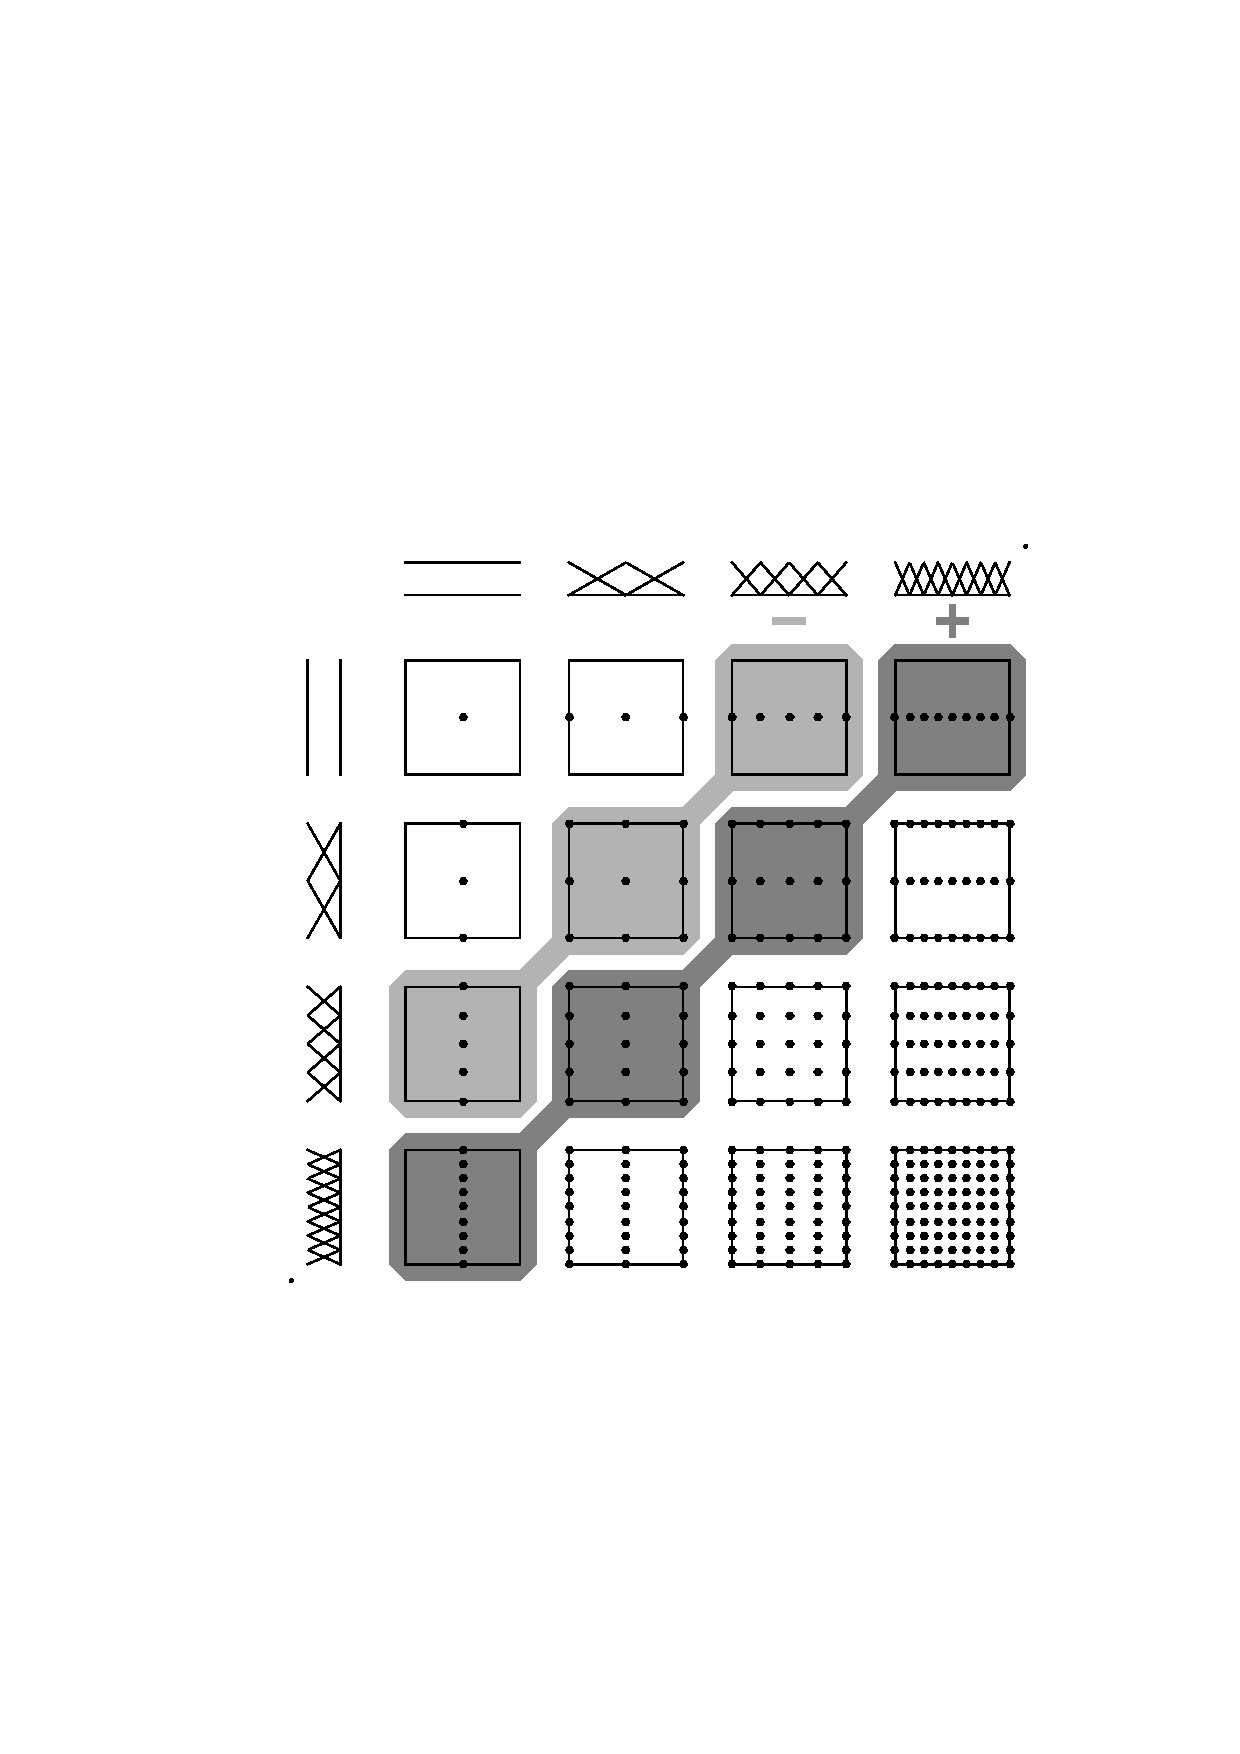
\includegraphics[width=1.1\textwidth]{combination_linear.png}


\end{column}

\end{columns}

\end{frame}
%--------------------------------------------------------------------------

%------------------------------------------------------------- Frame ------
\begin{frame}\frametitle{Combination Formula}

\begin{equation*}
\bar u_{m}(\boldsymbol{\xi})  \overset{\text{def}}{=}  \sum_{k=0}^{d-1}(-1)^{k}\binom{d-1}{k}\sum_{|\underline{i}|=m-k}u_{\underline{i}}(\boldsymbol{\xi}) .
\end{equation*}



\begin{columns}
\begin{column}{0.4\textwidth}
In the 2 D case
\begin{gather*}
\bar u_{m}(\boldsymbol{\xi})  \overset{\text{def}}{=}  \\
\sum_{|\underline{i}|=m}u_{\underline{i}}(\boldsymbol{\xi})  
 - \sum_{|\underline{i}|=m-1}u_{\underline{i}}(\boldsymbol{\xi}) .
\end{gather*}
\end{column}

\begin{column}{0.6\textwidth}

\centering
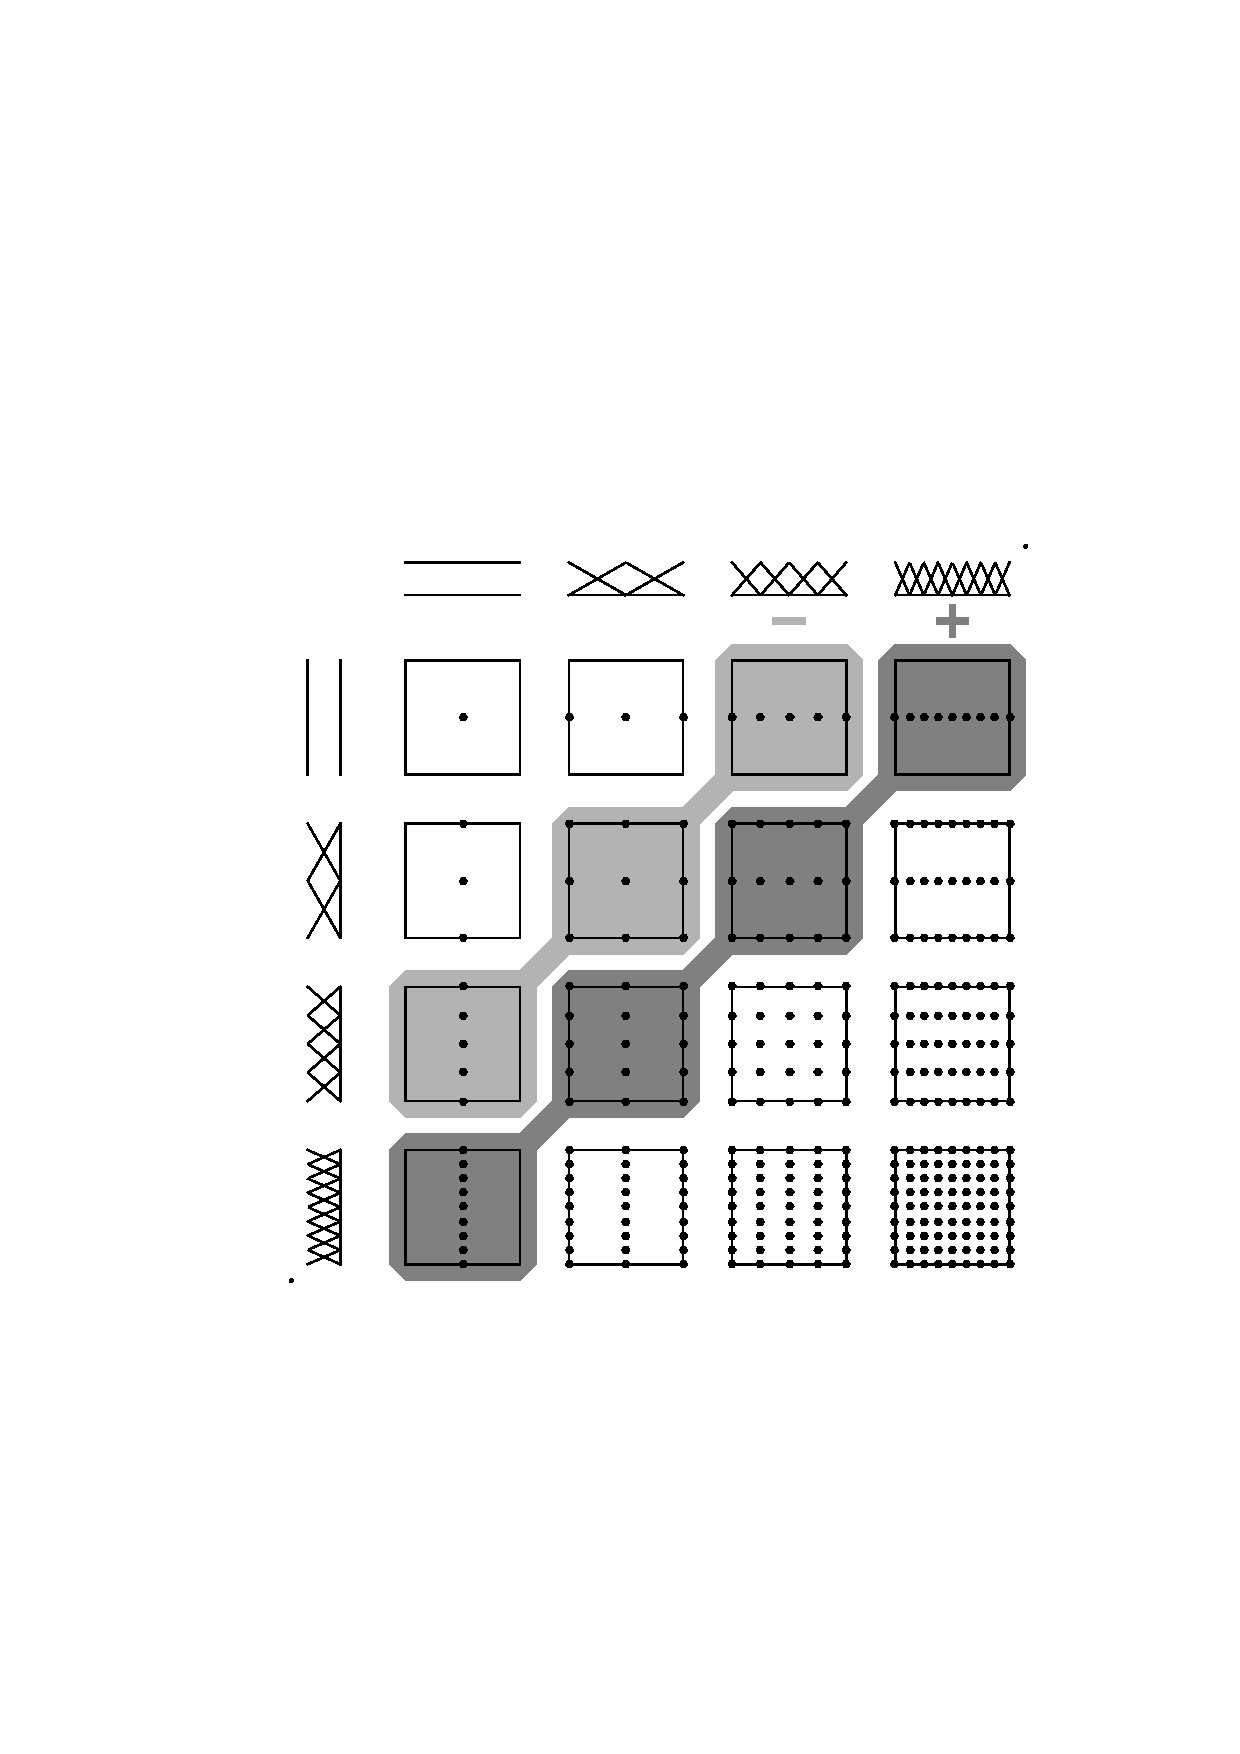
\includegraphics[width=1.1\textwidth]{combination_linear.png}


\end{column}

\end{columns}


%

\end{frame}
%--------------------------------------------------------------------------

%------------------------------------------------------------- Frame ------
\begin{frame}\frametitle{Multi-Fidelity Sparse Grid}

\begin{itemize}
\item Suppose we have two sparse grid interpolants,\\
$\bar u_m^\text{HF}({\boldsymbol{\xi}})$ for our high-fidelity simulation and \\
$\bar u_n^\text{LF}({\boldsymbol{\xi}})$ for our low-fidelity simulation. 

\item This is a useful approach if we aim to reduce the number of high-fidelity simulations by having $m<n$. 

\item We use the combination method  to combine our interpolants
%
\begin{equation*}
\bar u_{m,n}^\text{MF}(\boldsymbol{\xi})  \overset{\text{def}}{=} \bar u_m^\text{HF}(\boldsymbol{\xi})  + \bar u_n^\text{LF}(\boldsymbol{\xi})  - \bar u_m^\text{LF}(\boldsymbol{\xi}) ,
\end{equation*}



\item $\bar u_{m,n}^\text{MF}(\boldsymbol{\xi})$ the multi-fidelity interpolant, 

\item $\bar u_m^\text{HF}(\boldsymbol{\xi})$ the interpolant of the high-fidelity process sampled on the coarse sparse grid, 

\item $\bar u_n^\text{LF}(\boldsymbol{\xi})$ the interpolant of the low-fidelity process sampled on the fine sparse grid 

\item $\bar u_m^\text{LF}(\boldsymbol{\xi})$ the interpolant of the low-fidelity process sampled on the coarse sparse grid. 


\end{itemize}

\end{frame}
%--------------------------------------------------------------------------


%------------------------------------------------------------- Frame ------
\begin{frame}%\frametitle{Multi-Fidelity Sparse Grid}


\begin{center}
\includegraphics[width=0.8\textwidth]{combination_multifi}
\end{center}

The open circles (on the left) denote low-fidelity simulations, the closed circles (on the right) are high-fidelity simulations.  

The high-fidelity fine sparse grid interpolant on the bottom-right is approximated by the combination of the sparse grid interpolants three cheaper grids. 


\end{frame}
%--------------------------------------------------------------------------


%------------------------------------------------------------- Frame ------
\begin{frame}\frametitle{Multi-Fidelity Sparse Grid}

\begin{itemize}
\item We can rewrite as
%
\begin{equation*}
\bar u_{m,n}^\text{MF}(\boldsymbol{\xi})  \overset{\text{def}}{=} \bar u_n^\text{LF}(\boldsymbol{\xi})  + \bar d_m(\boldsymbol{\xi}) ,
\end{equation*}
%
with
%
\begin{equation*}
\bar d_m(\boldsymbol{\xi}) \overset{\text{def}}{=} \bar u_m^\text{HF}({\boldsymbol{\xi}}) - \bar u_m^\text{LF}({\boldsymbol{\xi}}) .
\end{equation*}
%
\item
Here $\bar d_m$ is interpolant of the difference process sampled on the coarse sparse grid. 

\item The assumption that we make is that the difference process is a relatively smooth function of the input parameters, such that it can be represented on the coarse sparse grid.


\end{itemize}

\end{frame}
%--------------------------------------------------------------------------



%------------------------------------------------------------- Frame ------
\begin{frame}\frametitle{Example}

A one-dimensional illustration of the multifidelity approach.

\begin{center}
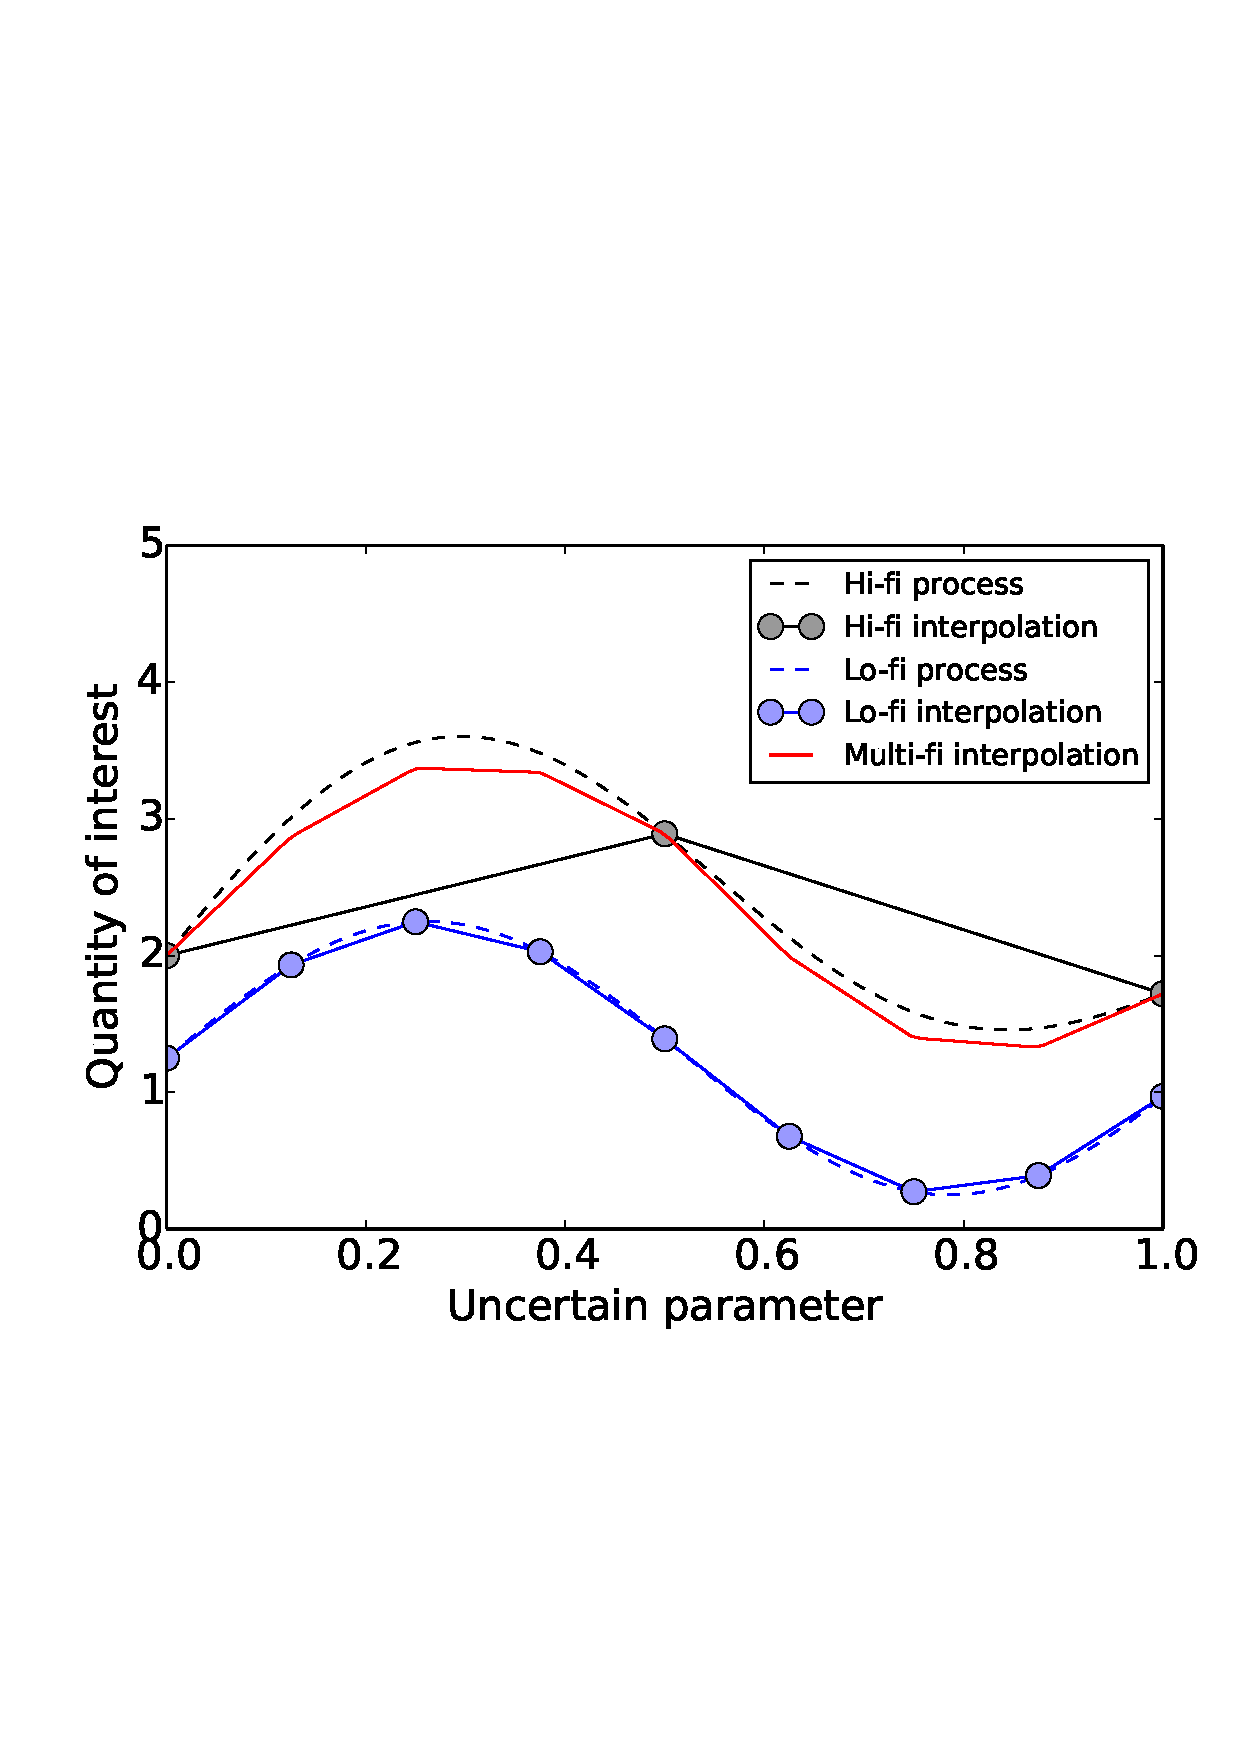
\includegraphics[width=0.8\textwidth]{method2}
\end{center}


\end{frame}
%--------------------------------------------------------------------------




%------------------------------------------------------------- Frame ------
\begin{frame}\frametitle{Tsunami Runup Example}

\begin{itemize}
\item  Simulation Software ANUGA

\item Velocity correction

\item Results


\end{itemize}

\end{frame}
%--------------------------------------------------------------------------


%------------------------------------------------------------- Frame ------
\begin{frame}\frametitle{Modelling tsunamis with ANUGA}

\begin{itemize}
\item ANUGA is a fluid dynamics module
which uses the finite-volume method to  solve the Shallow Water
Wave Equations.

\item Can model the process of
wetting and drying as water enters and leaves an area.

\item User specifies the geometry
(bathymetry and topography), the initial water level (stage),
boundary conditions such as incoming tsunami waves, and any operators  that may
drive the system such as rainfall, abstraction of water,  erosion, culverts

\item Most ANUGA  components are written in the object-oriented programming
language Python.   

\item Computationally intensive components are written for
efficiency in C routines working directly with Python \mbox{numpy
structures.}

\end{itemize}

\end{frame}
%--------------------------------------------------------------------------









%------------------------------------------------------------- Frame ------
\begin{frame}\frametitle{Okushiri Tsunami Case Study}


\begin{center}
\includegraphics[width=0.8\textwidth]{tsunami-aonae}
\end{center}

{\small Tsunami and related fire damage at Aonae, SE Okushiri Island, Japan.
More than 120 people were killed in Japan (Okushiri and Hokkaido
Islands) by the 1993 tsunami.}

\vfill



\end{frame}
%--------------------------------------------------------------------------



%------------------------------------------------------------- Frame ------
\begin{frame}\frametitle{Okushiri Tsunami Case Study}


\begin{center}
\includegraphics[width=0.6\textwidth]{okushiri-location.jpg}

\end{center}

\end{frame}
%--------------------------------------------------------------------------

%------------------------------------------------------------- Frame ------
\begin{frame}\frametitle{Okushiri Tsunami Case Study}


\begin{center}

\includegraphics[width=0.6\textwidth]{okushiri-wave-heights.jpg}

\end{center}

\end{frame}
%--------------------------------------------------------------------------


%------------------------------------------------------------- Frame ------
\begin{frame}\frametitle{Validation Scenario}

\begin{columns}
\begin{column}{0.6\textwidth}
\begin{center}
\includegraphics[width=\textwidth]{monai-contour.pdf}
\end{center}
\end{column}

\begin{column}{0.4\textwidth}
\begin{itemize}
\item Benchmark Scenario \#2 selected from 3rd Int'l Workshop on LWRU
2004

\vspace{0.25cm}
\item Tsunami Run-up onto a Complex Three-dimensional  Beach.

\vspace{0.25cm}
\item 1/400 scale laboratory experiment of the Monai run-up (Okushiri
Island, Japan, 1993).
\end{itemize}
\end{column}
\end{columns}

\end{frame}
%--------------------------------------------------------------------------





%------------------------------------------------------------- Frame ------
\begin{frame}\frametitle{Experimental Setup}


\begin{center}
\includegraphics[width=\textwidth]{experimental-setup}
\end{center}

\end{frame}
%--------------------------------------------------------------------------




%------------------------------------------------------------- Frame ------
\begin{frame}\frametitle{Experiment Overhead view}


\begin{center}
\includemedia[
     addresource=monai-experiment-overhead-slow.mp4,
     flashvars={
          src=monai-experiment-overhead-slow.mp4%
          &autoPlay=true}]
   {\includegraphics[width=\textwidth]{monai-experiment-overhead}}
   {StrobeMediaPlayback.swf}
\end{center}

\end{frame}
%--------------------------------------------------------------------------

%------------------------------------------------------------- Frame ------
\begin{frame}\frametitle{Simulation Overhead view}

\begin{center}
\includemedia[
     addresource=monai-simulation-overhead-slow.mp4,
     flashvars={
          src=monai-simulation-overhead-slow.mp4%
          &autoPlay=true}]
   {\includegraphics[width=\textwidth]{monai-simulation-overhead}}
   {StrobeMediaPlayback.swf}
\end{center}

\end{frame}
%--------------------------------------------------------------------------





%------------------------------------------------------------- Frame ------
\begin{frame}\frametitle{Okishiri Benchmark}
 
\begin{itemize}

\item This Okushiri experiment is now considered a standard benchmark test-case for tsunami prediction. 

\item We focus on the time-dependent average height of the water layer on top of the Monai valley, our area of interest. 

\item We assume that the total energy of the prescribed incoming wave is known, but that it's exact shape is uncertain.
\end{itemize}

\end{frame}
%--------------------------------------------------------------------------

%------------------------------------------------------------- Frame ------
\begin{frame}\frametitle{Computational Domain and Area of Interest}

\begin{center}
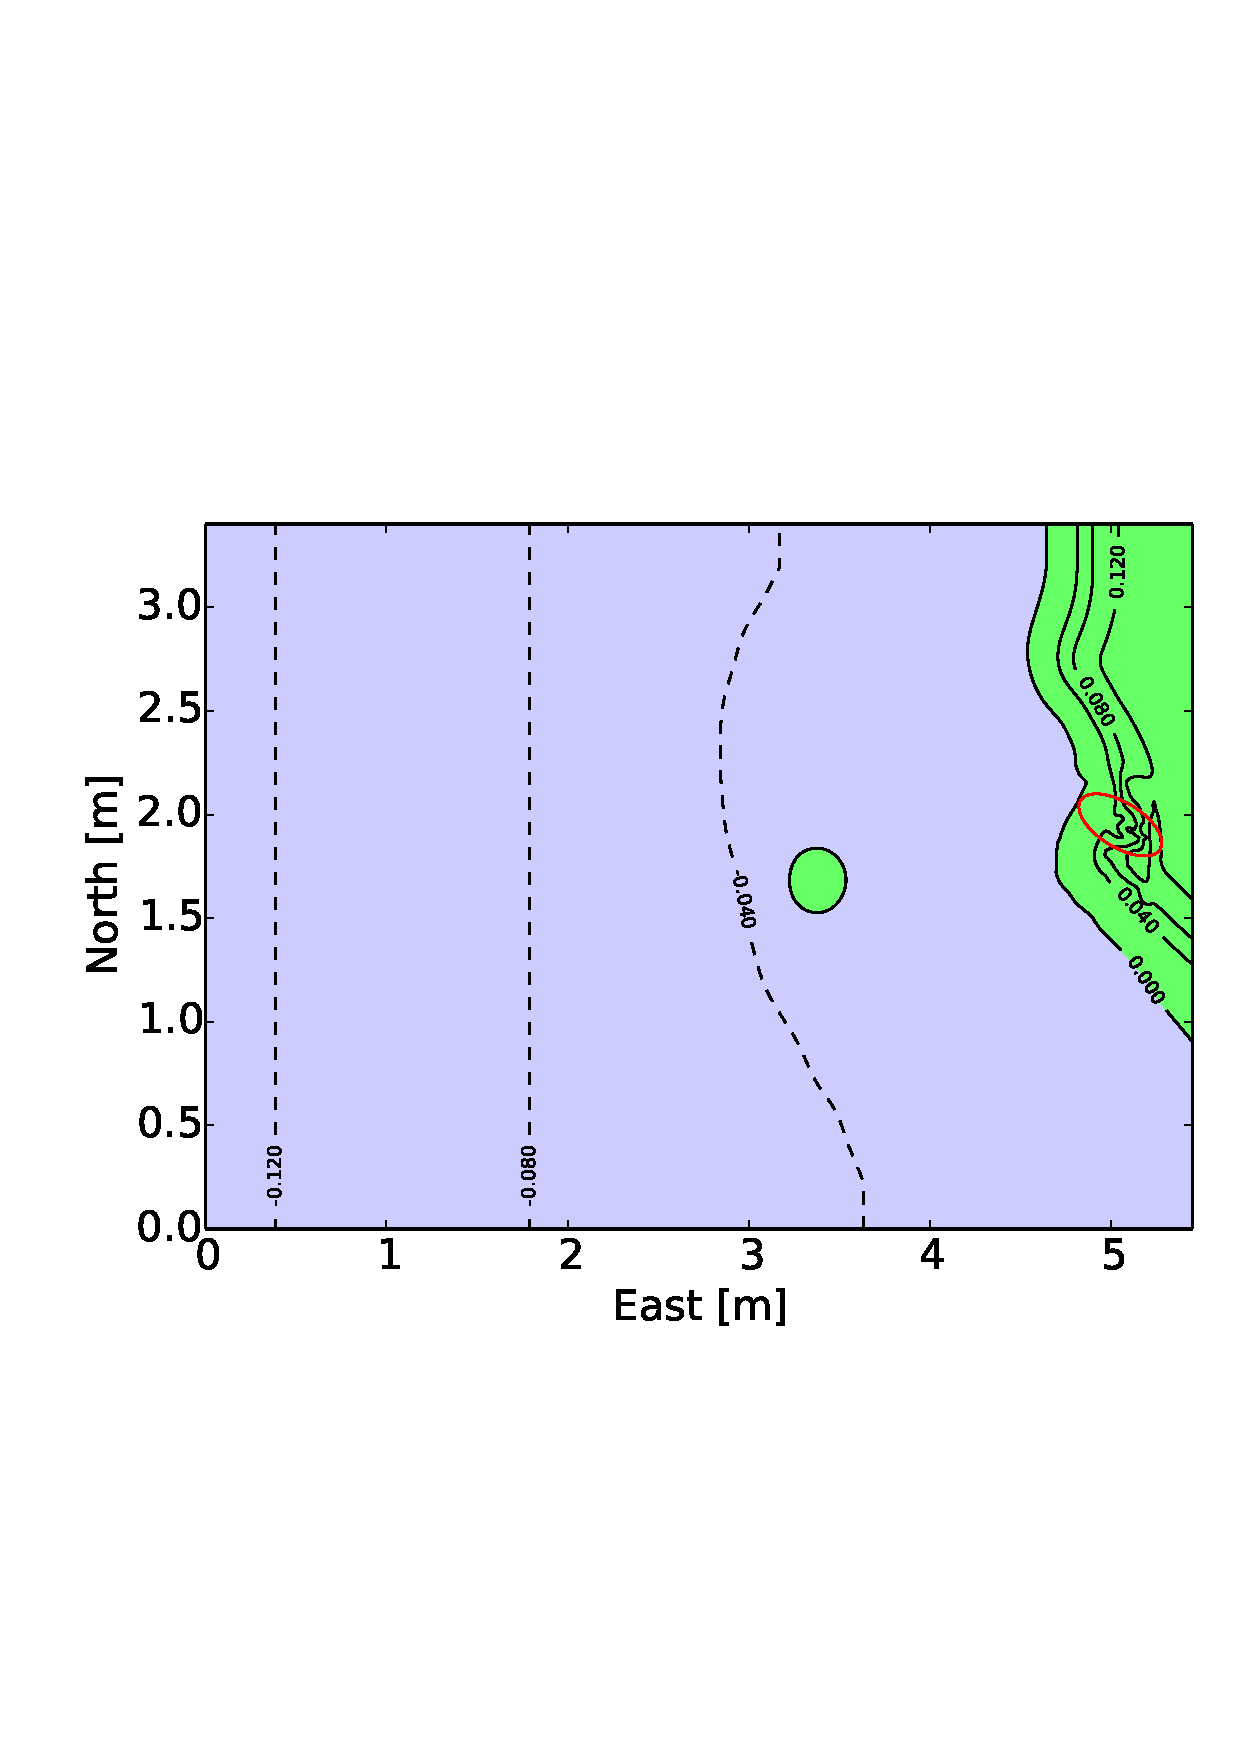
\includegraphics[width=0.7\textwidth]{problem_setup_geometry}
\end{center}


\small{
The computational domain. The wave comes in from the left, the area of interest is indicated by the ellipse on the right. The quantity of interest is the average water level in the area of interest, as a function of time. }

\end{frame}
%--------------------------------------------------------------------------

%------------------------------------------------------------- Frame ------
\begin{frame}\frametitle{Computational Mesh}

\begin{center}
\includegraphics[width=0.4\textwidth]{problem_setup_mesh_64}\textsf{(a)}
\includegraphics[width=0.4\textwidth]{problem_setup_mesh_256}\textsf{(b)}
\end{center}

\small{
Examples of the computational mesh, for (a) $64$ and (b) $256$ cells. The mesh is refined around the area of interest. In our simulations we use meshes of $262,\!114$ and $16,\!384$ cells for the high-fidelity and low-fidelity simulations, respectively.}

\end{frame}
%--------------------------------------------------------------------------

%------------------------------------------------------------- Frame ------
\begin{frame}\frametitle{Runup Wave}

\begin{center}
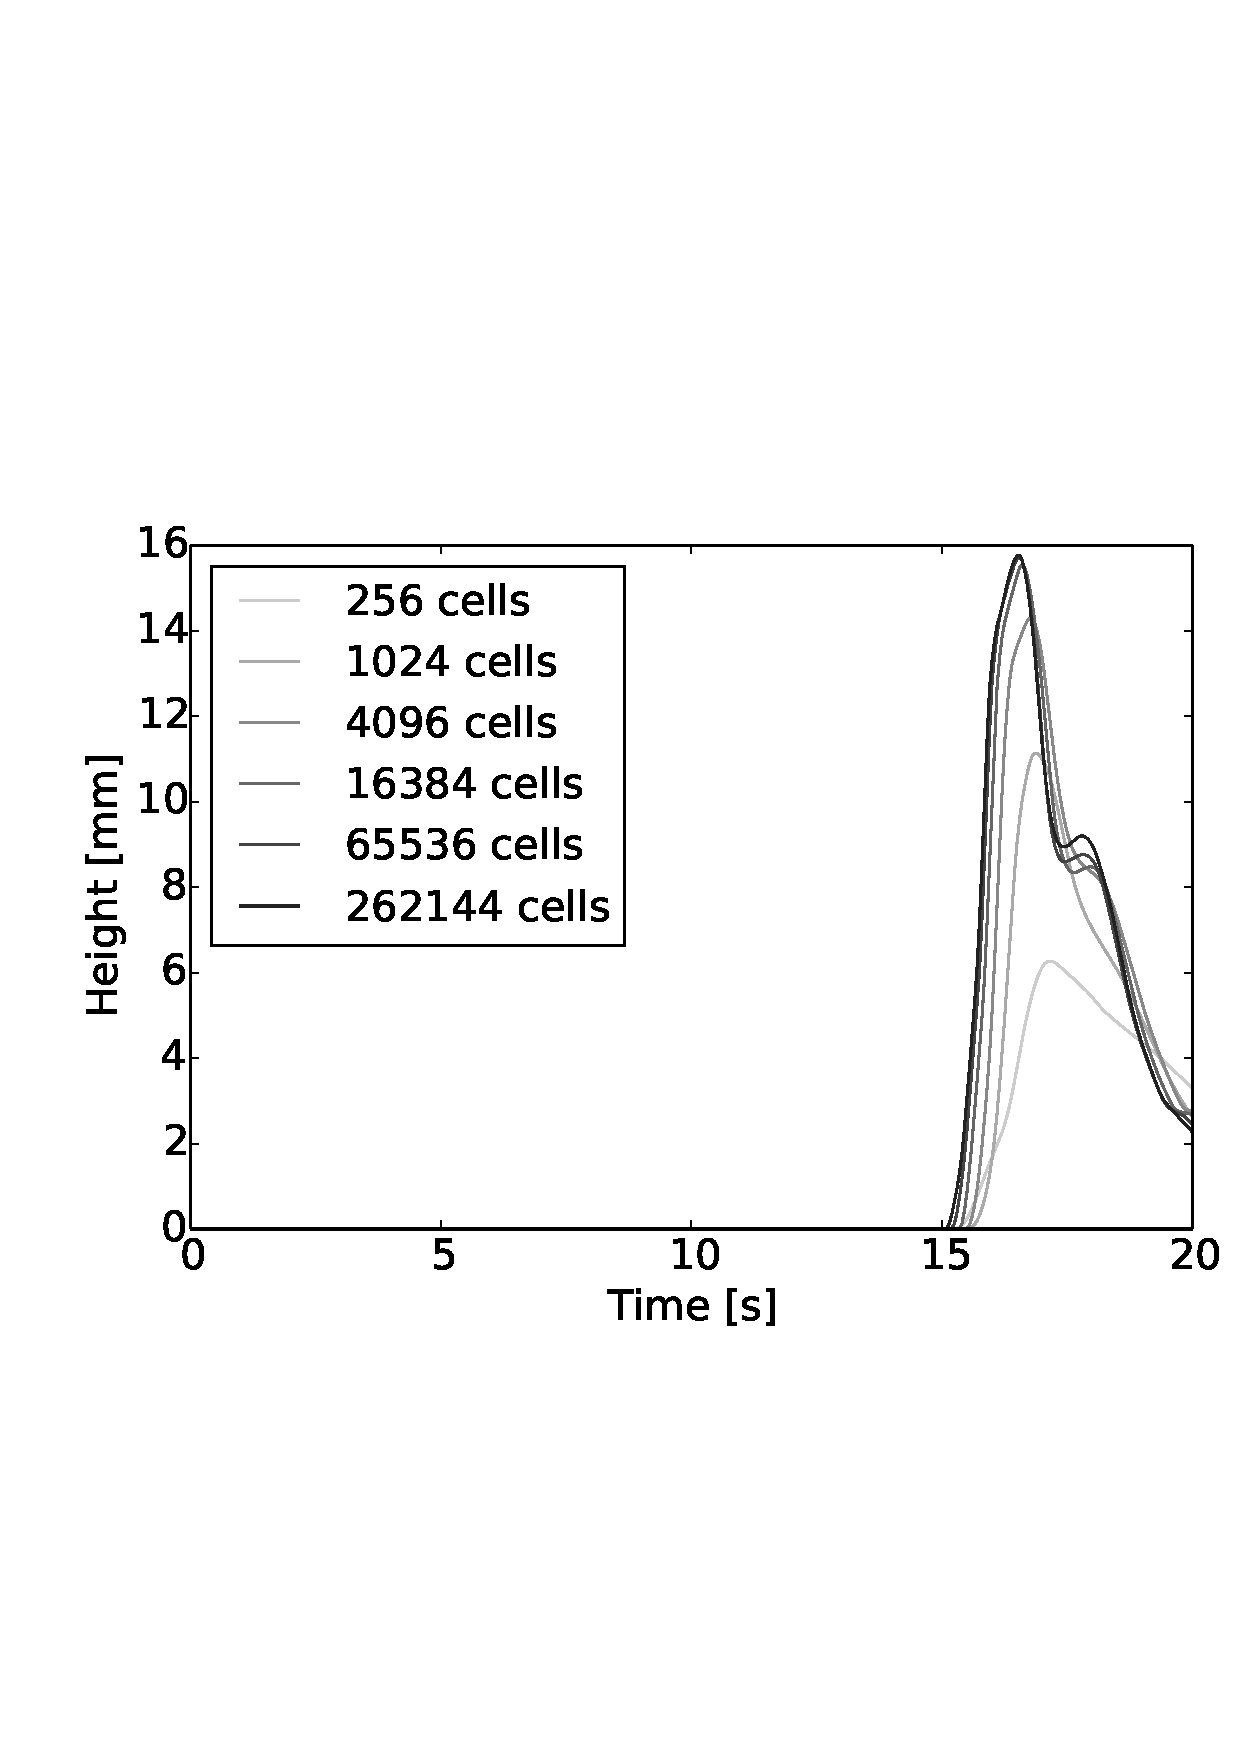
\includegraphics[width=0.7\textwidth]{mesh_convergence_height}
\end{center}


\small{
The average water level in the area of interest as a function of time. The result converges as the mesh gets finer. Note that  the wave arrives earlier for finer meshes. In our simulations we use meshes of $262,\!114$ and $16,\!384$ cells for the high-fidelity and low-fidelity \mbox{simulations, respectively.}}



\end{frame}
%--------------------------------------------------------------------------

%------------------------------------------------------------- Frame ------
\begin{frame}\frametitle{Computational Time}

\begin{center}
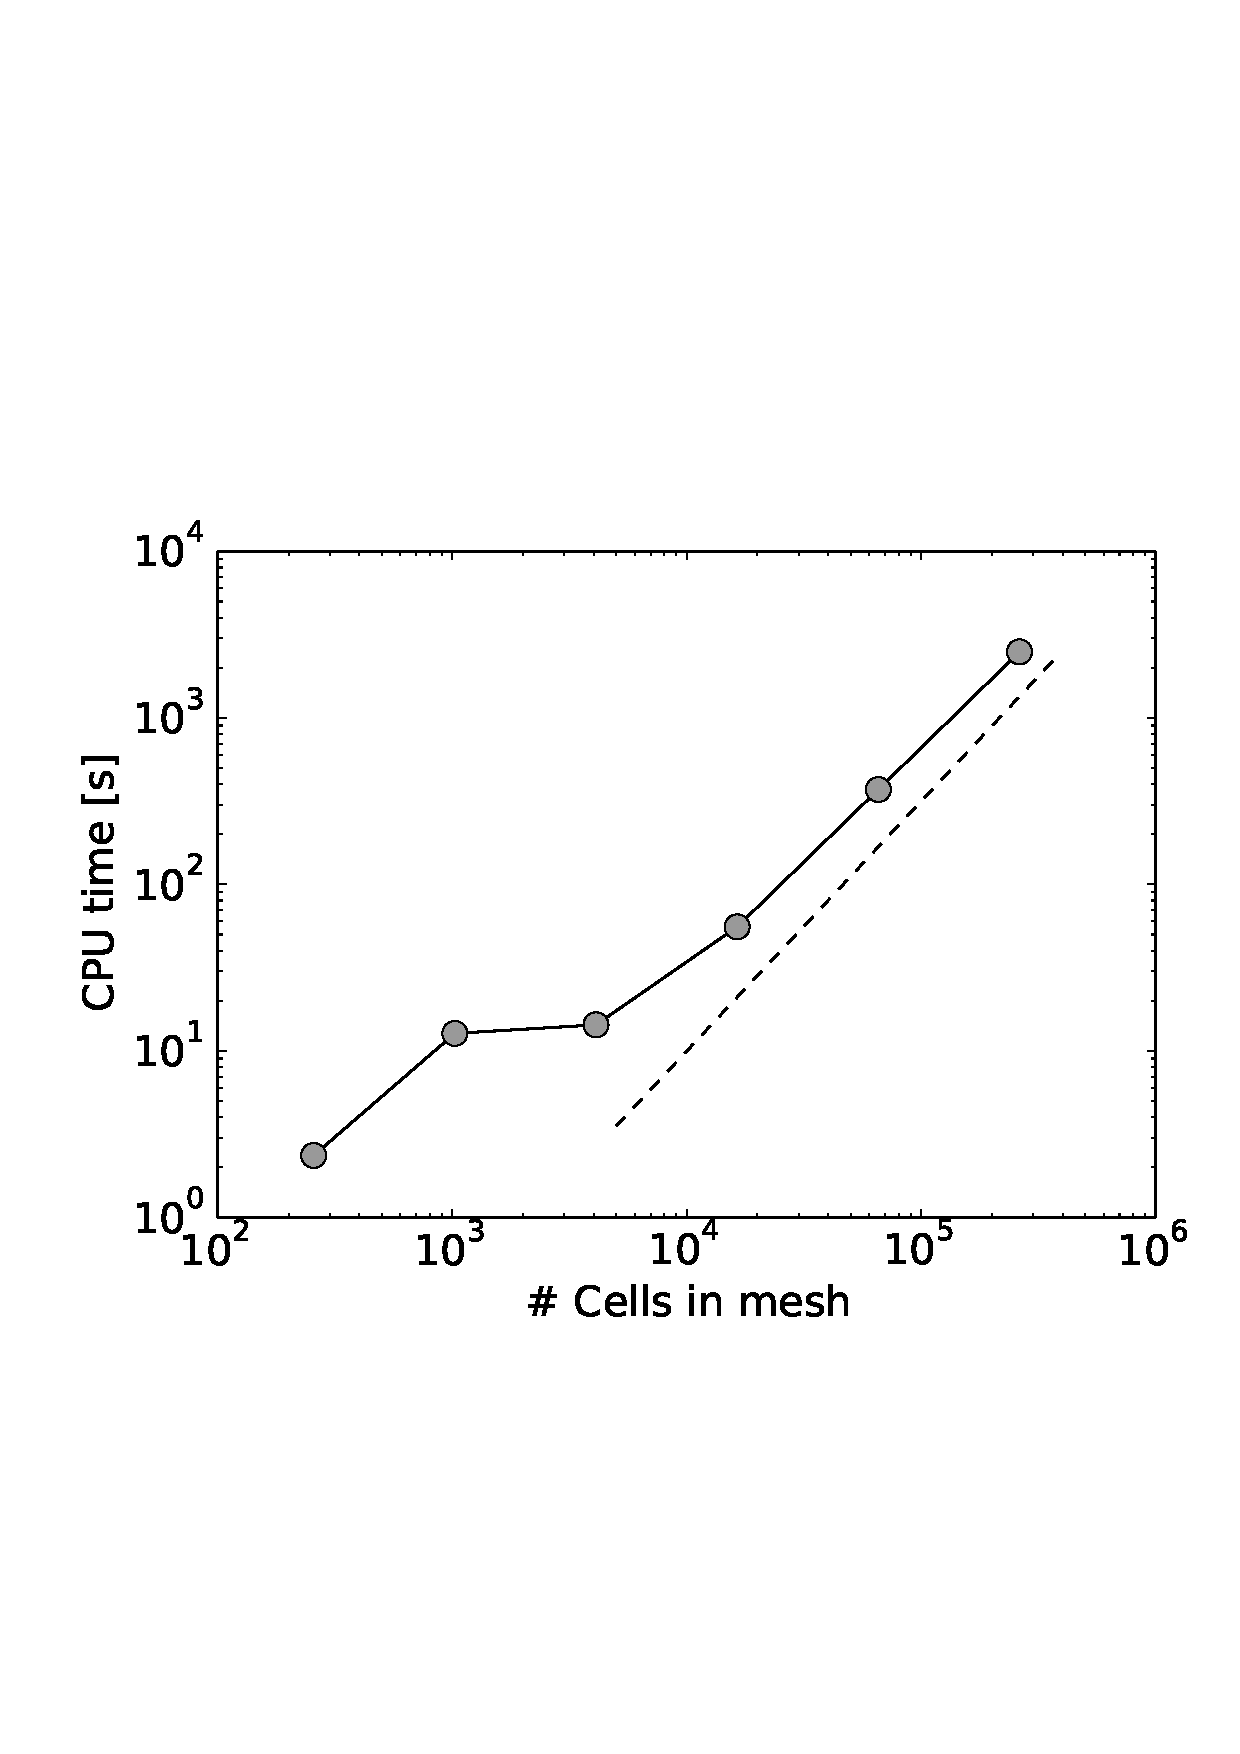
\includegraphics[width=0.7\textwidth]{mesh_convergence_time}
\end{center}

\small{
The CPU time required for running a simulation increases with the number of cells in the mesh. The dashed line represents the expected rate of increase. CPU timings are on an Intel Core i$5$ \mbox{$2.80$ GHz processor.}}

\end{frame}
%--------------------------------------------------------------------------

%------------------------------------------------------------- Frame ------
\begin{frame}\frametitle{Parametrised Incoming Wave}

\begin{center}
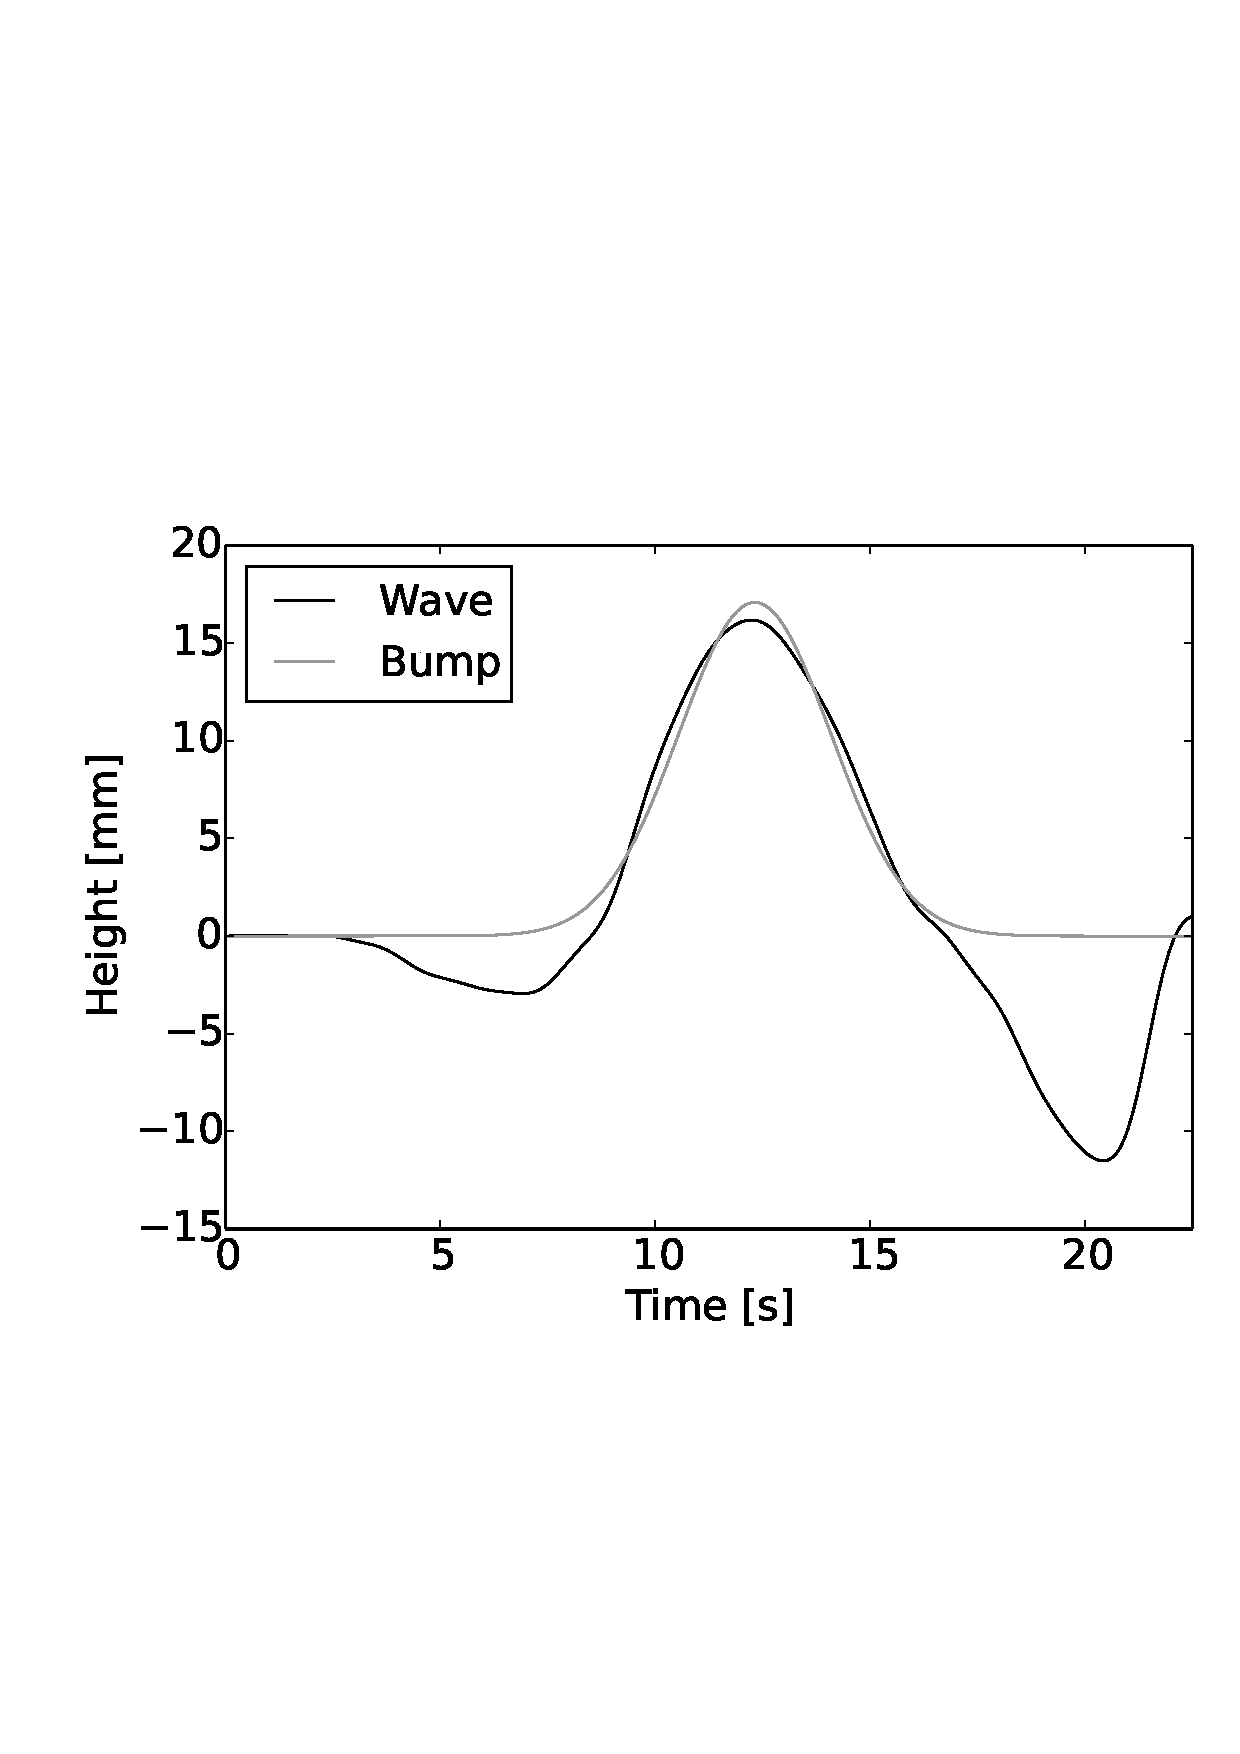
\includegraphics[width=0.7\textwidth]{parametrisation_bump}
\end{center}

\small{
Fitting the deterministic incoming wave with a single Gaussian bump. To represent an increasing number of uncertain input parameters, we fit a sequence of bumps.}

\end{frame}
%--------------------------------------------------------------------------

%------------------------------------------------------------- Frame ------
\begin{frame}\frametitle{Parametrised Incoming Wave}

\begin{center}
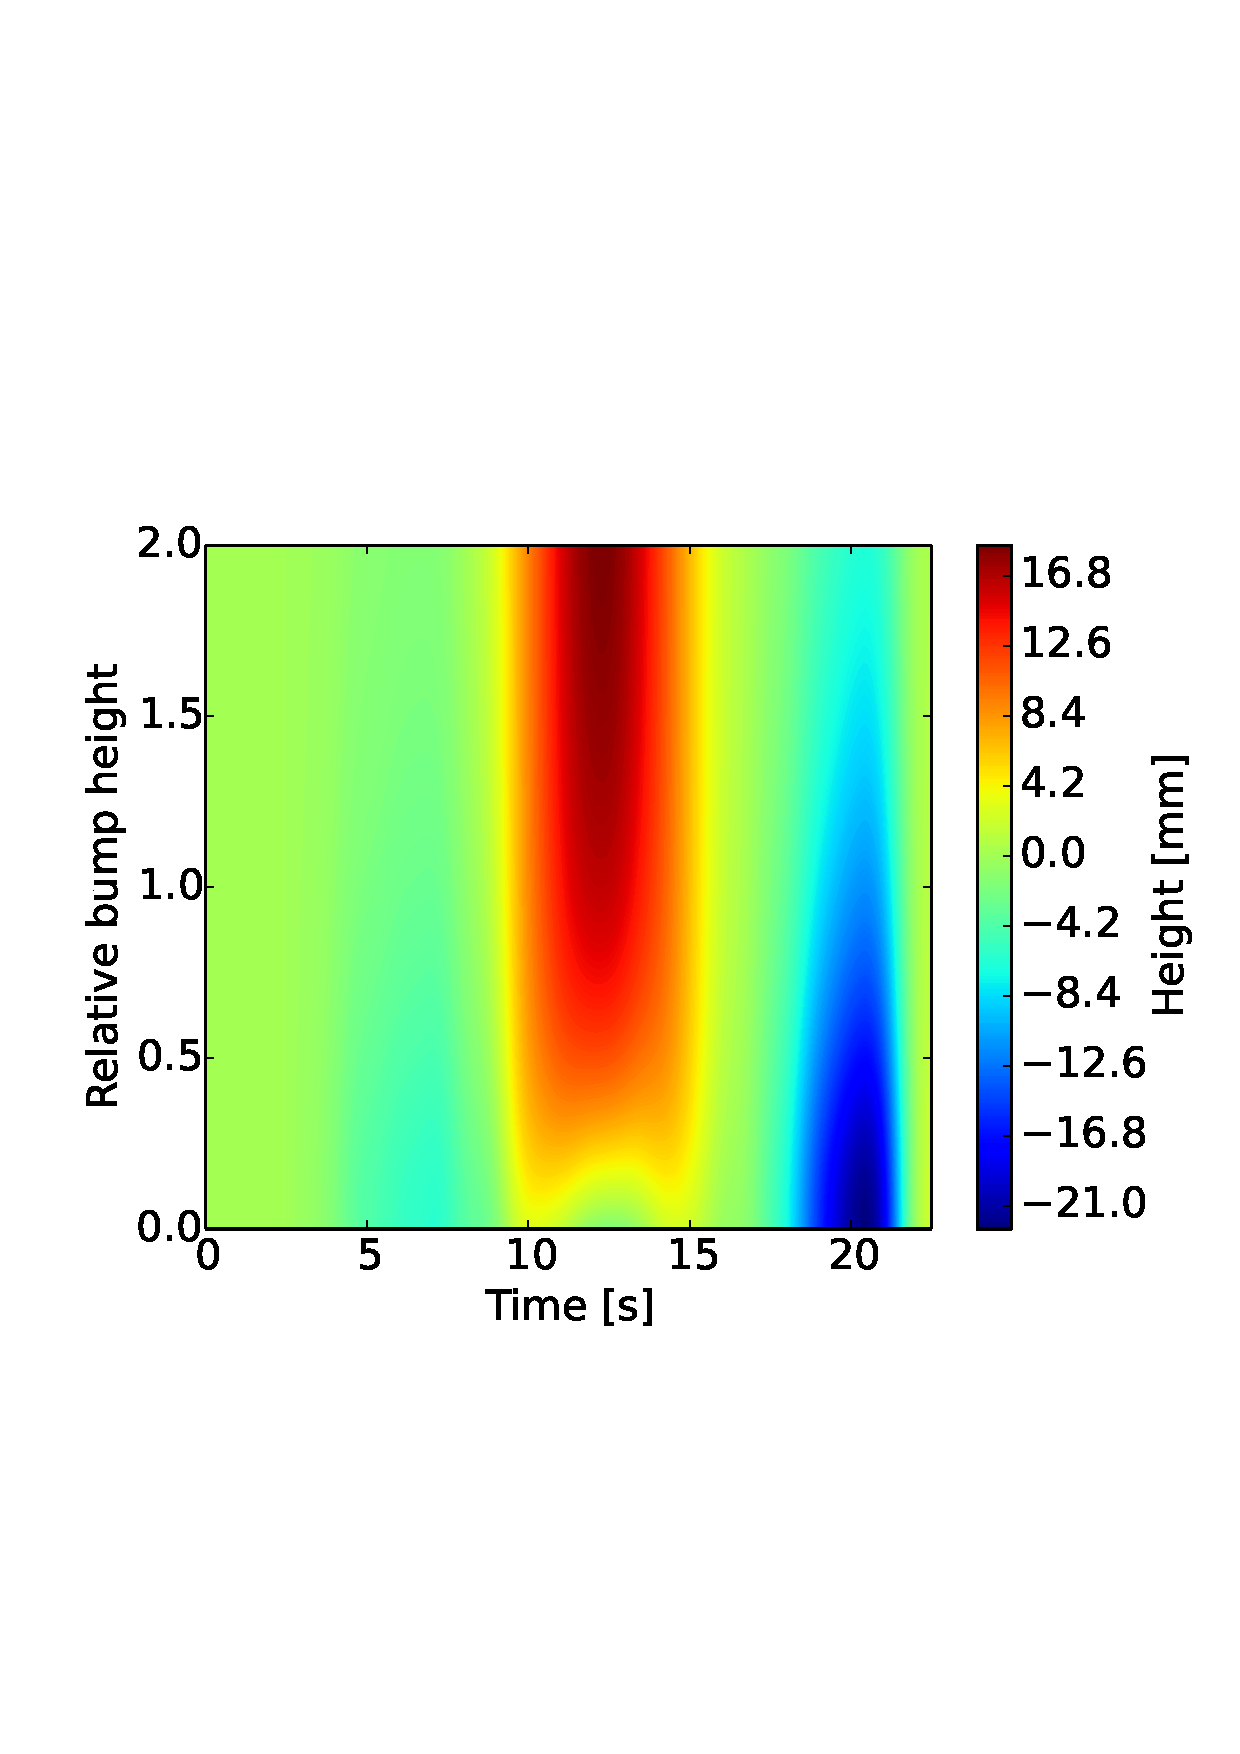
\includegraphics[width=0.7\textwidth]{illustrate1d_incoming_wave}
\end{center}

\small{
The incoming wave as a function of time and of the untransformed relative bump height. The incoming wave is parametrised by a single bump, with a maximum around $12$ s. 

Note that when the height of this bump is decreased, the bump at around $20$ s grows, because we keep the total energy of the incoming wave constant.}


\end{frame}
%--------------------------------------------------------------------------




%------------------------------------------------------------- Frame ------
\begin{frame}\frametitle{High and Low Fidelity Output}

\begin{center}
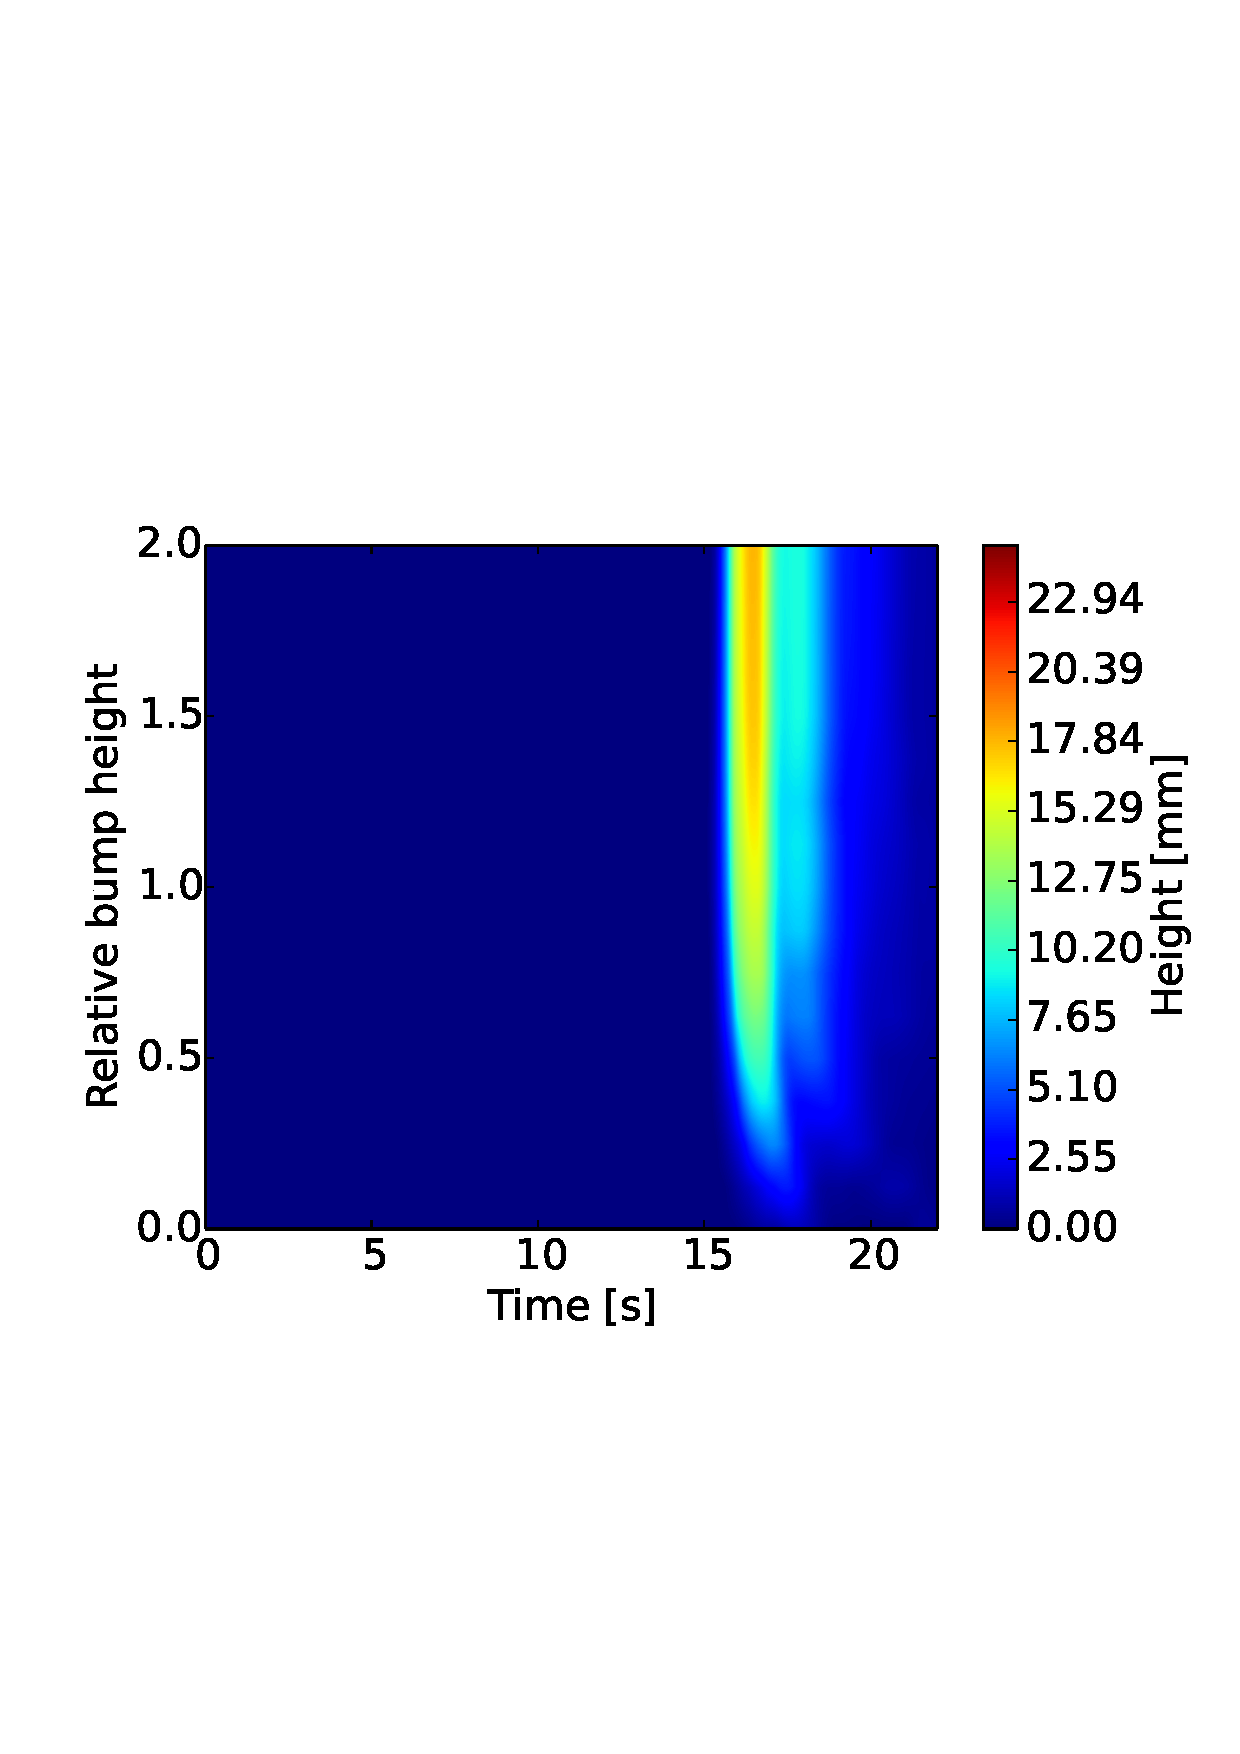
\includegraphics[width=0.4\textwidth]{illustrate1d_data_hf}\textsf{(a)}
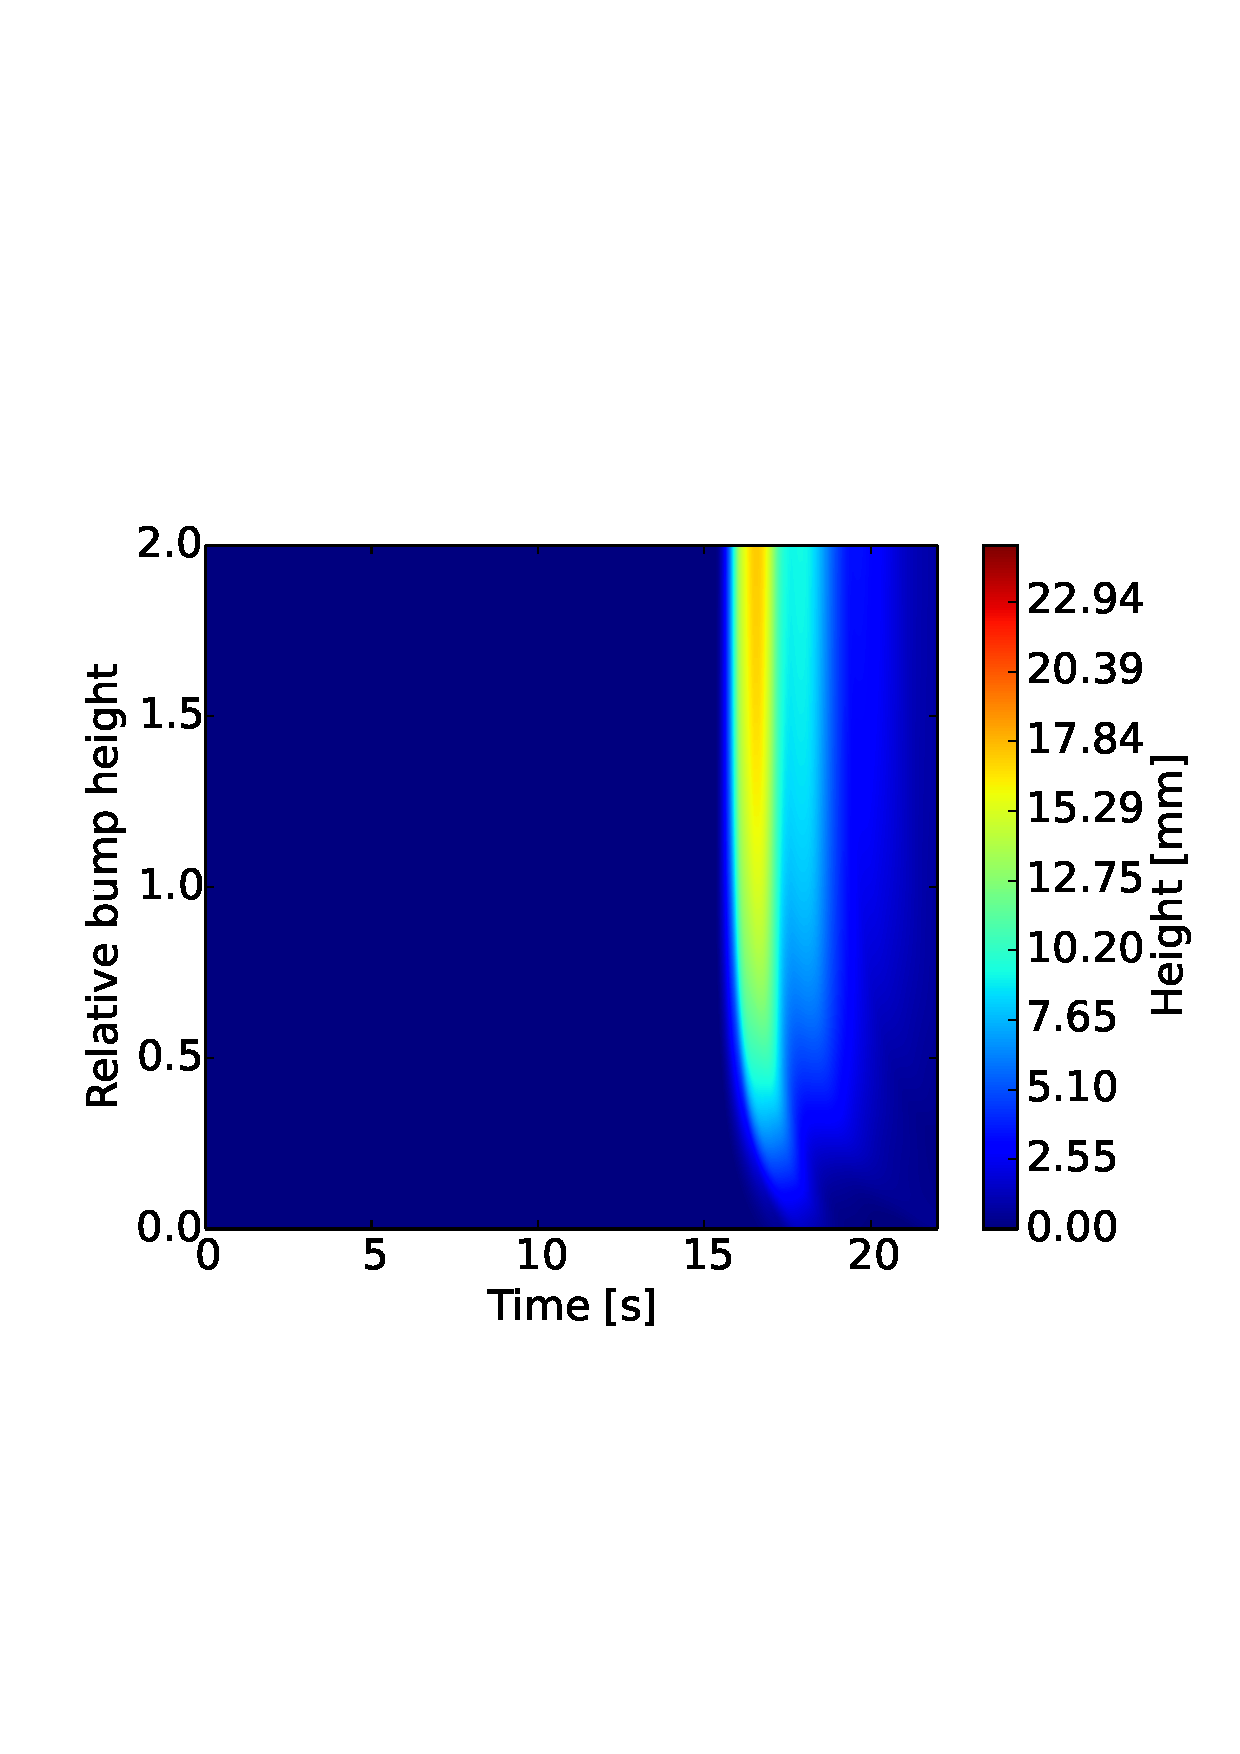
\includegraphics[width=0.4\textwidth]{illustrate1d_data_lf}\textsf{(b)}
\end{center}

\small{
The (a) high-fidelity and (b) low-fidelity output of our code, as a function of time and of the untransformed relative bump height. Decreasing the height of the main bump in the incoming wave leads to a smaller maximum in the output. The low-fidelity signal is somewhat delayed with respect to the high-fidelity signal. (More clear from the next slide.)}


\end{frame}
%--------------------------------------------------------------------------


%------------------------------------------------------------- Frame ------
\begin{frame}\frametitle{Differences}

\begin{center}
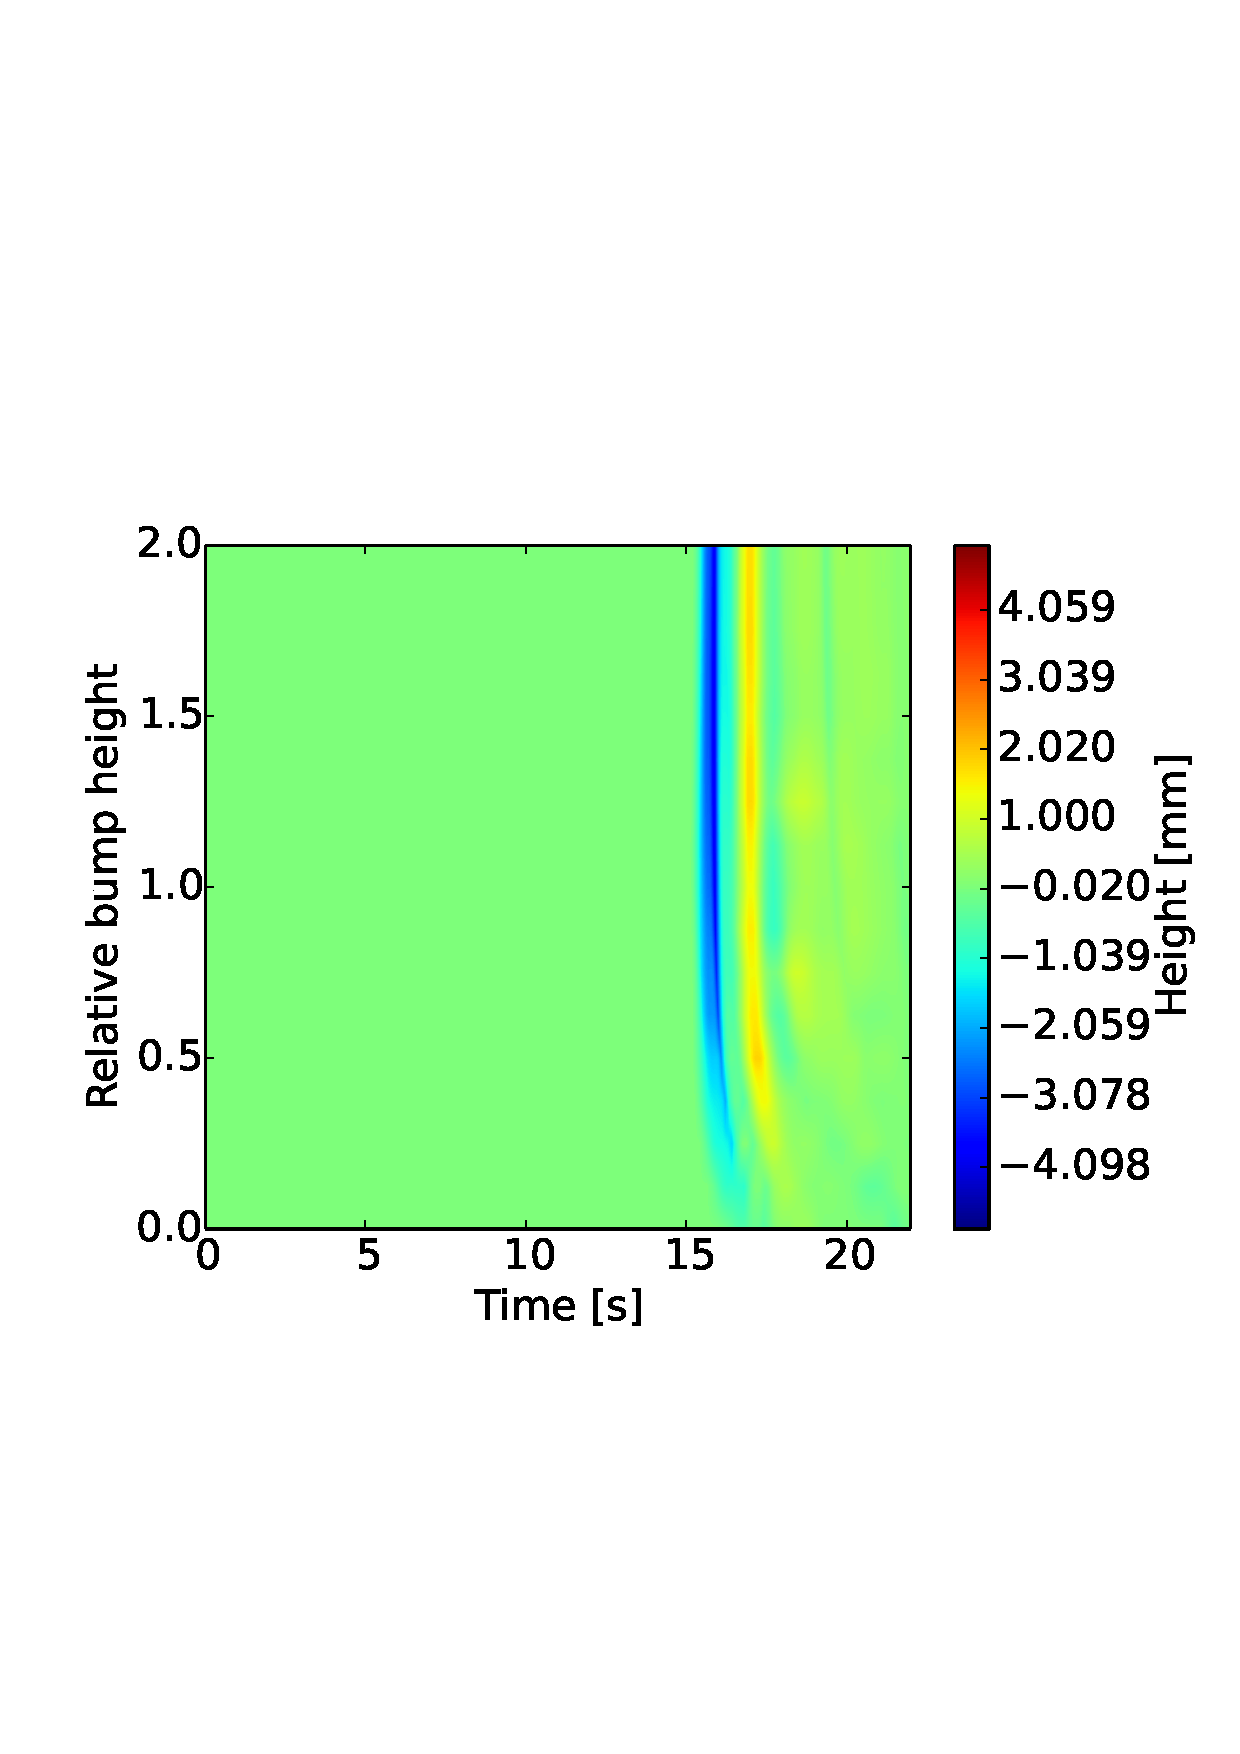
\includegraphics[width=0.4\textwidth]{illustrate1d_difference1}\textsf{(a)}
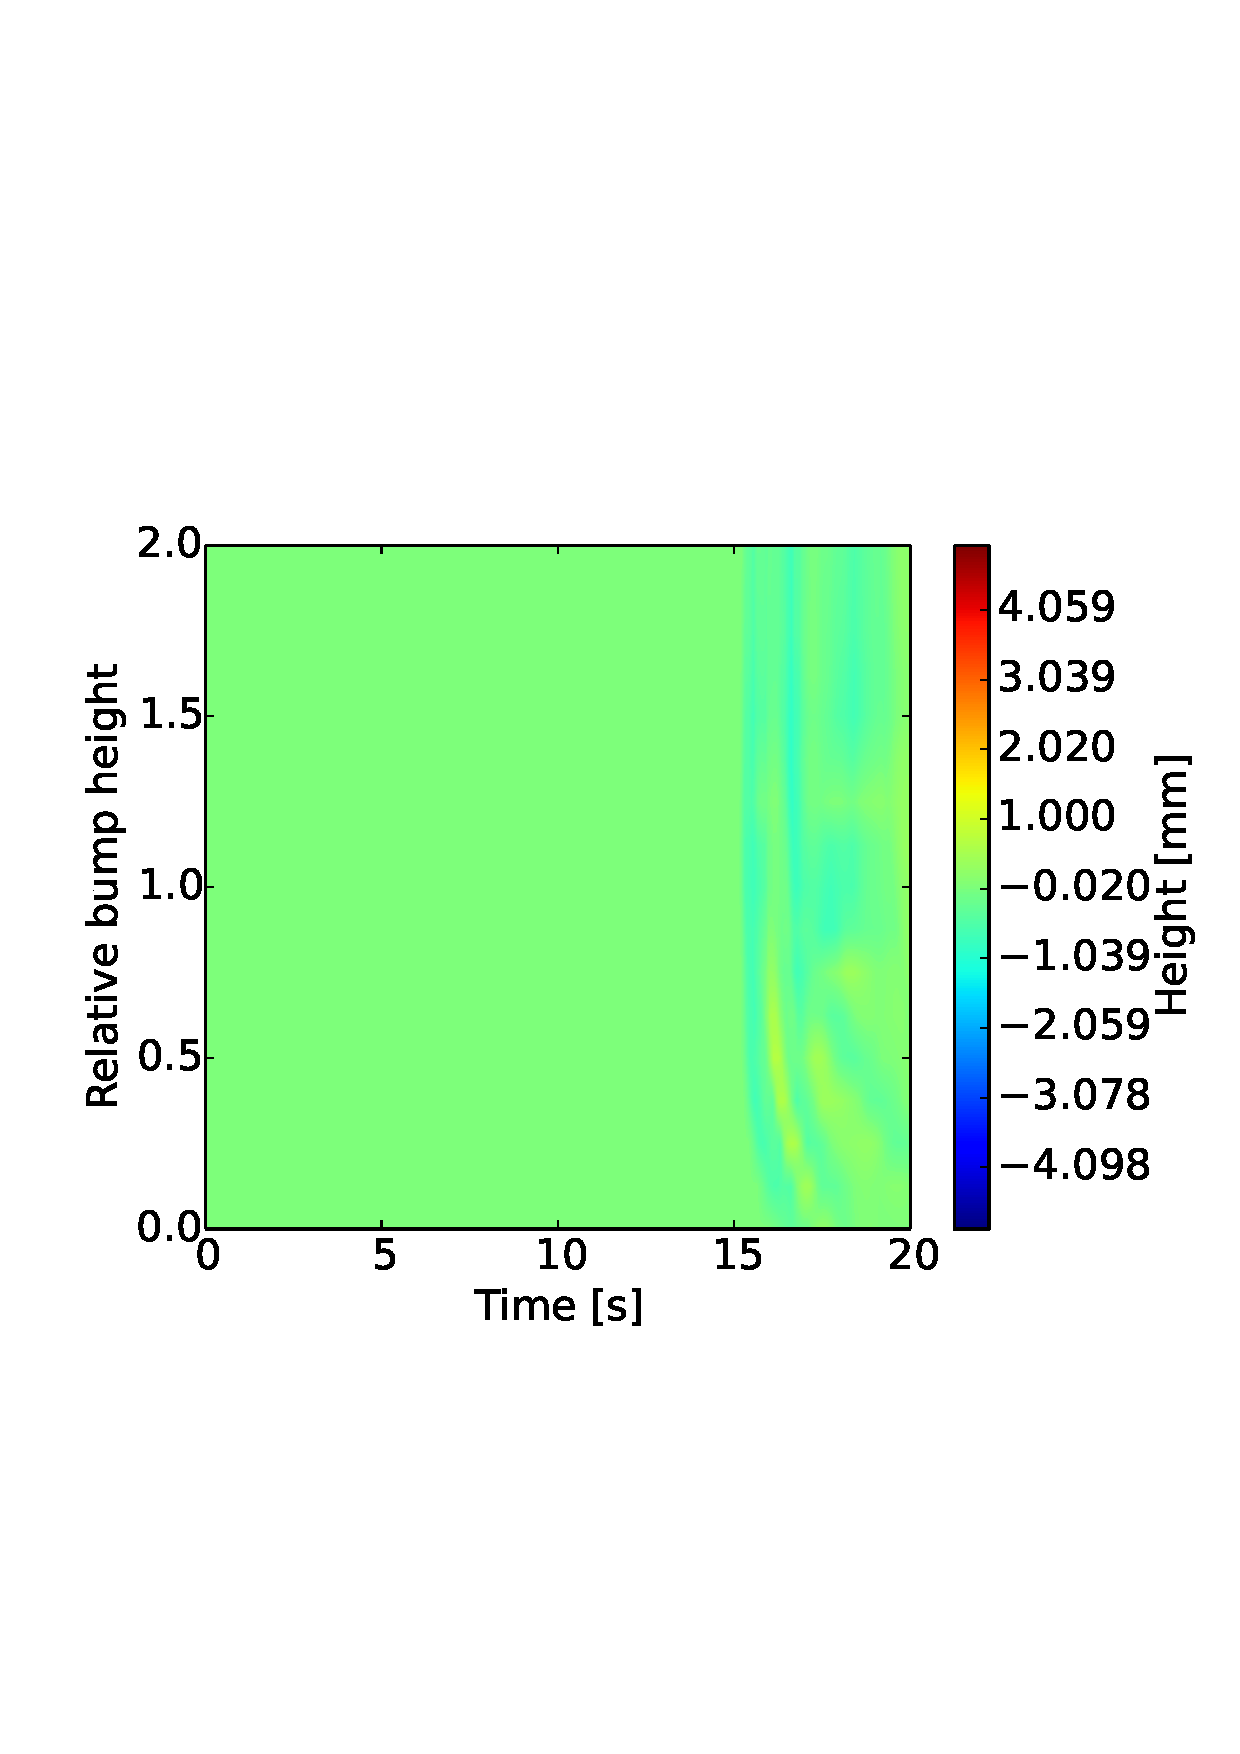
\includegraphics[width=0.4\textwidth]{illustrate1d_difference2}\textsf{(b)}
\end{center}

\small{
(a) The difference between the low-fidelity and high-fidelity results from previous Figure. (b) The difference after scaling of the time for the low-fidelity result, thus correcting for the lower speed of the wave on the coarse mesh. After scaling, the difference is a much smoother function of the relative bump height, which is a requirement for the application of multifidelity sparse grid interpolation. The time scaling is further illustrated in the next slide.}


\end{frame}
%--------------------------------------------------------------------------

%------------------------------------------------------------- Frame ------
\begin{frame}\frametitle{Correcting the Wave Velocity}

\begin{itemize}
\item From our computer experiments we find that the wave velocity depends on the size of the computational mesh. 

\item We correct for this by scaling the time in the result of the low-fidelity simulation. 

\item The corrected low-fidelity result is given by
%
\begin{equation}
u_{\text{corr}}^\text{LF}(\boldsymbol{\xi})(t) = u_{\text{raw}}^\text{LF}(\boldsymbol{\xi})(c t),
\end{equation}
%

\item The time correction factor $c$ is found from
%
\begin{equation}
c = \text{ arg } \underset{c}{\text{min }}  \int_{t=0}^{t=20}| u_{\text{raw}}^\text{LF}(\boldsymbol{\xi})(c t) - u^\text{HF}(\boldsymbol{\xi})(t)|^2 \text{ d}t.
\end{equation}
%

\item $c$ is chosen such that it minimises the difference between the result of the low-fidelity and the high-fidelity simulation. 

\item $c$ is only available at the coarse sparse grid points, and so is interpolated using a coarse sparse grid. 

\item The assumption that we make is that the time correction is a relatively smooth function of the uncertain input parameters, such that we can represent it on the coarse sparse grid.


\end{itemize}

\end{frame}
%--------------------------------------------------------------------------


%------------------------------------------------------------- Frame ------
\begin{frame}\frametitle{Time Scaling}

\begin{center}
\includegraphics[width=0.7\textwidth]{illustrate1d_time_scaling}
\end{center}


\small{
The optimal time-scaling as a function of the relative bump height of the incoming wave. Note that we can only determine the time scaling factors where the high-fidelity simulations are available; for other relative bump heights we have to interpolate. }



\end{frame}
%--------------------------------------------------------------------------


%------------------------------------------------------------- Frame ------
\begin{frame}\frametitle{Comparison HF and MF}

\begin{center}
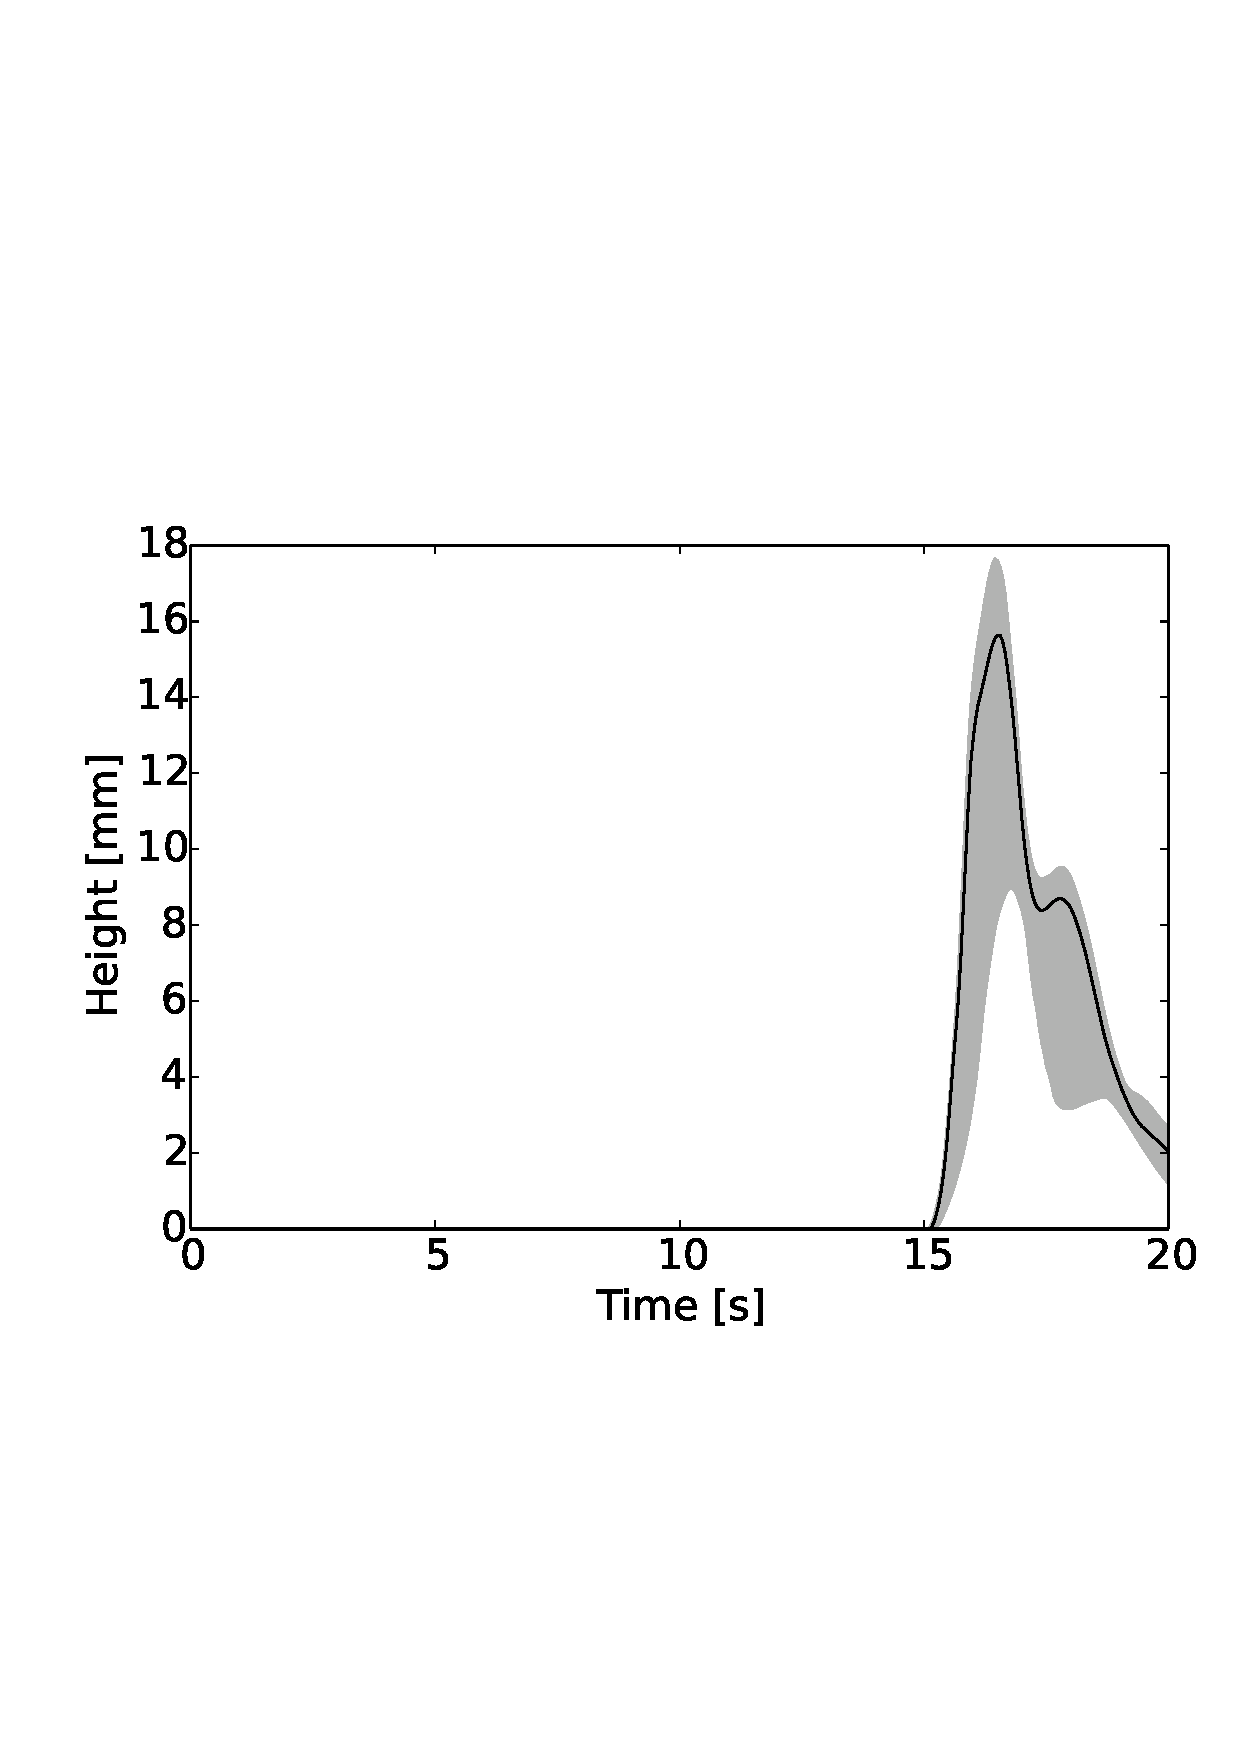
\includegraphics[width=0.4\textwidth]{illustrate1d_reference}\textsf{(a)}
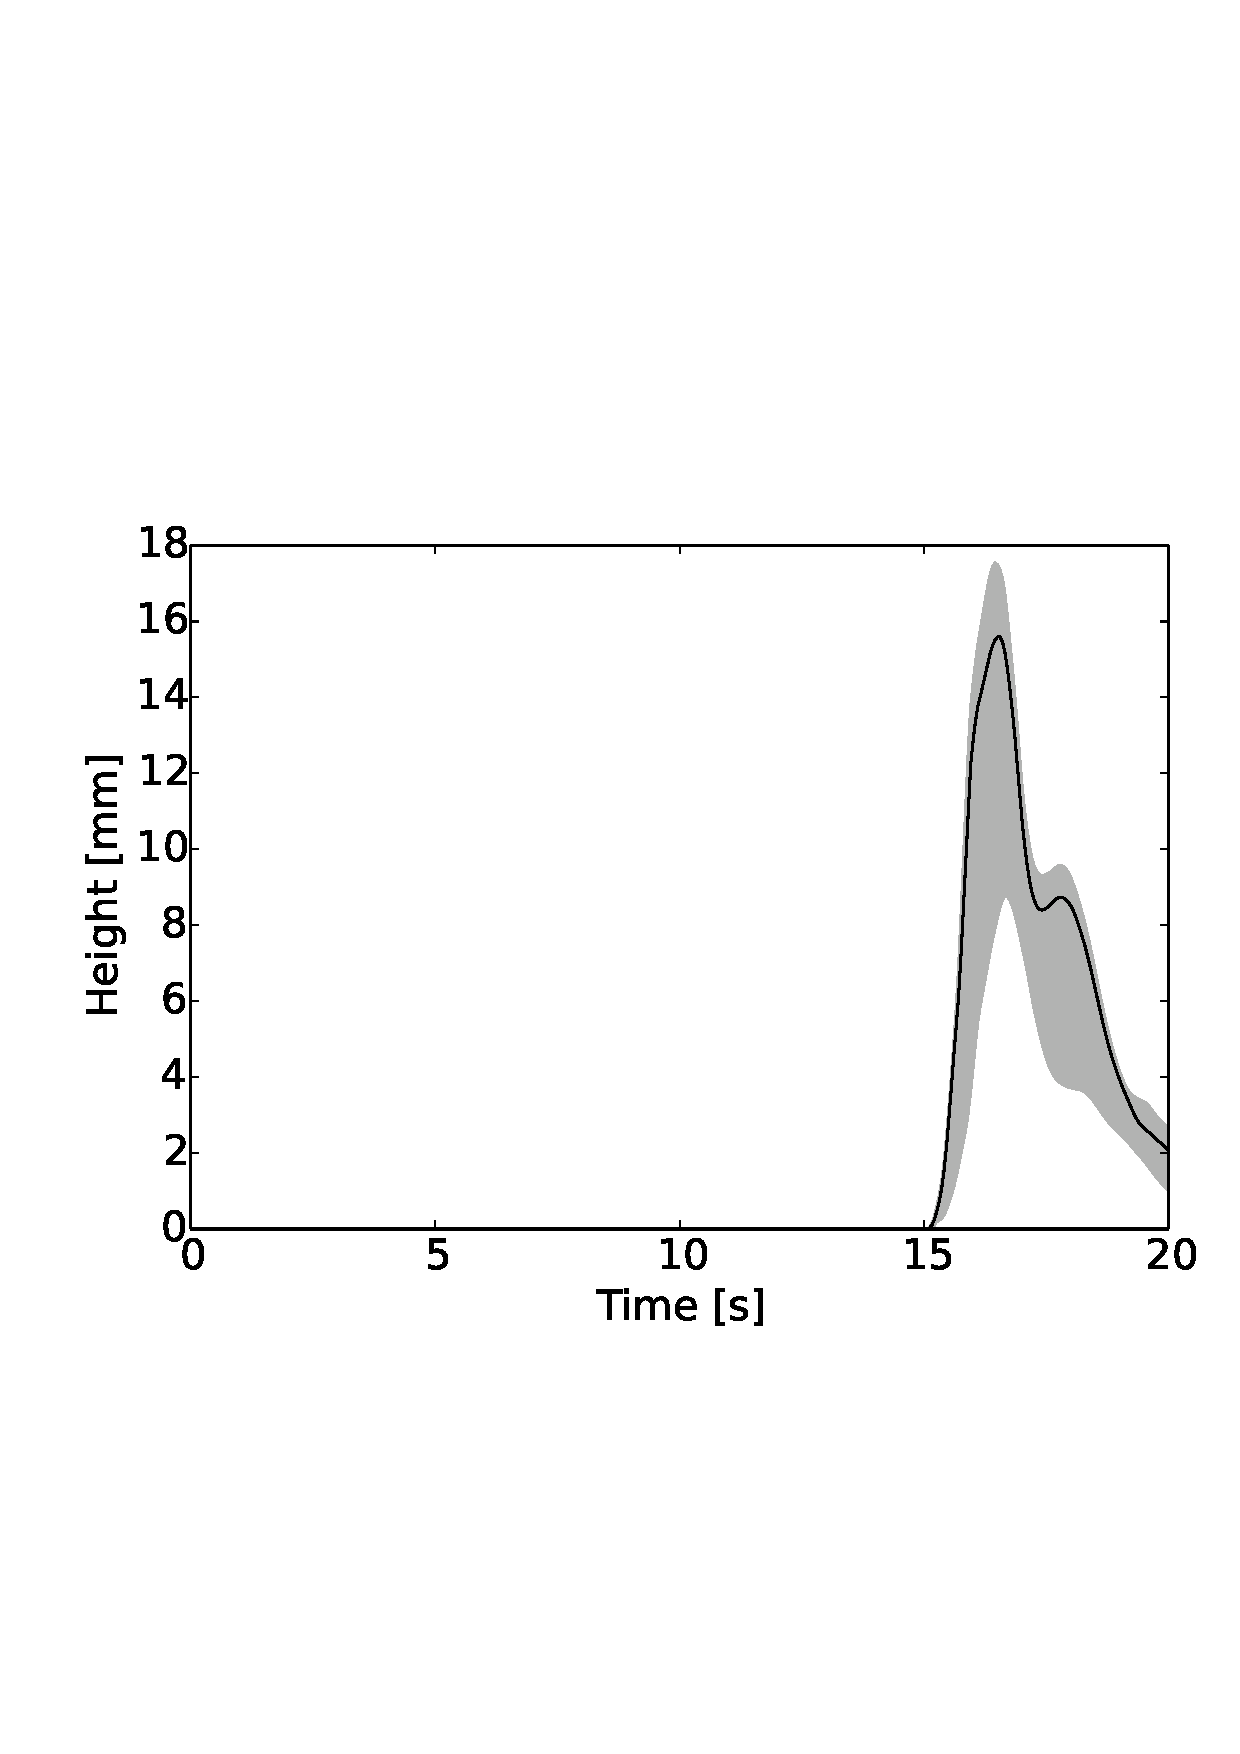
\includegraphics[width=0.4\textwidth]{illustrate1d_cheap}\textsf{(b)}
\end{center}

\small{
Uncertainty quantification for the result of our simulation, using 
(a) a large number of high-fidelity simulations as a reference result or 
(b) a multifidelity approach with three high-fidelity simulations and nine low-fidelity simulations. 

The multifidelity result is close to the reference result, which is further illustrated in the next slide.

The black line is the median, the gray area shows the $10\%$ and $90\%$ quantiles. }



\end{frame}
%--------------------------------------------------------------------------


%------------------------------------------------------------- Frame ------
\begin{frame}\frametitle{Convergence}

\begin{center}
\includegraphics[width=0.7\textwidth]{illustrate1d_converge}
\end{center}

\small{
The convergence of the high-fidelity and multifidelity results. Starting from a high-fidelity approach based on a certain number of simulations, we can add a larger number of low-fidelity simulations, following a dashed gray line. Depending on the desired level of accuracy, this multifidelity approach converges faster than the high-fidelity approach.}


\end{frame}
%--------------------------------------------------------------------------



%------------------------------------------------------------- Frame ------
\begin{frame}\frametitle{Convergence}

\begin{center}
\includegraphics[width=0.7\textwidth]{scaling}
\end{center}

\small{
The computational cost of accurate uncertainty quantification increases rapidly with the number of uncertain input parameters. Using a multifidelity approach mitigates this effect.

Using four random parameters, the normalised cost of the high-fidelity uncertainty quantification is $219$ simulations, compared to only $10$ simulations for the low-fidelity approach.}

\end{frame}
%--------------------------------------------------------------------------

%------------------------------------------------------------- Frame ------
\begin{frame}\frametitle{An 8 Dimensional Example}

\begin{center}
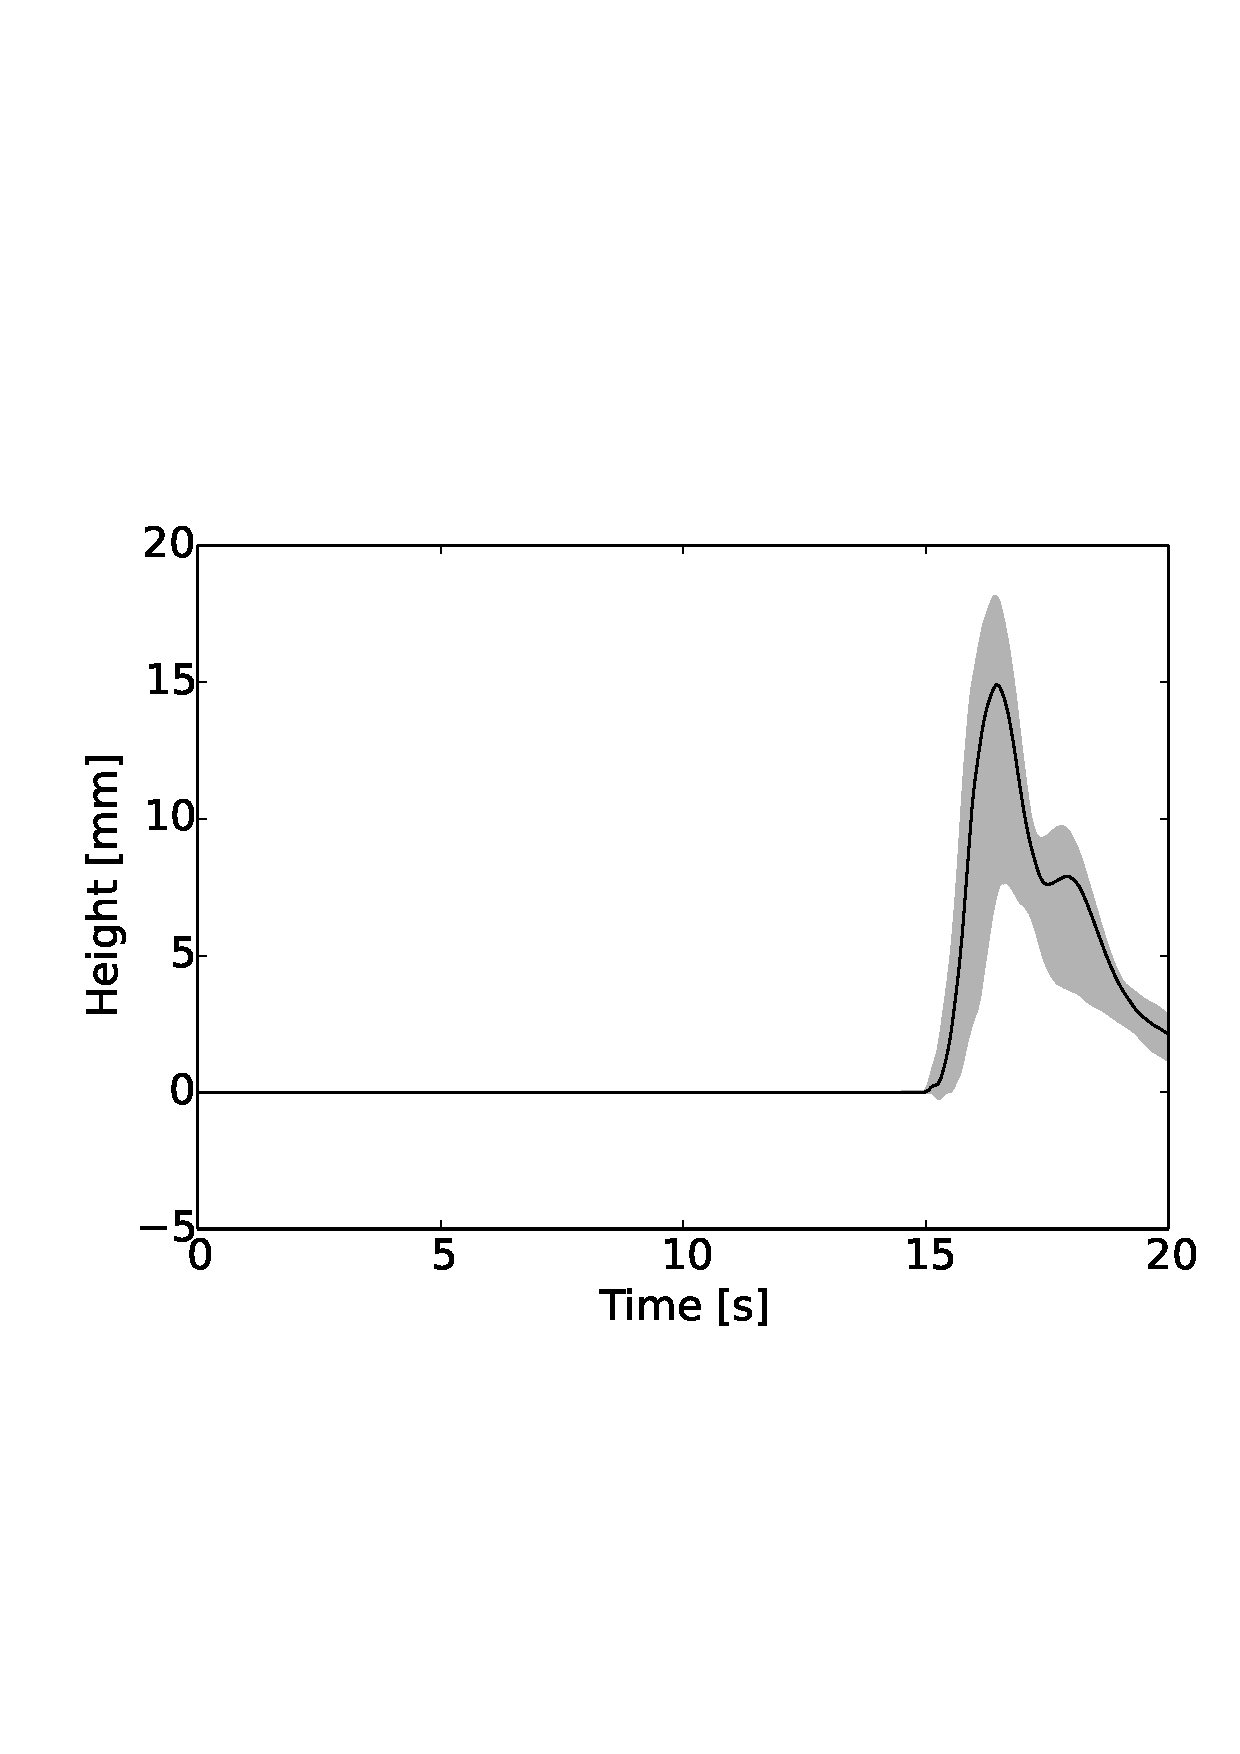
\includegraphics[width=0.7\textwidth]{full_problem}
\end{center}

\small{
Uncertainty quantification for the full problem, taking into account $8$ uncertain input parameters. The black line is the median, the gray area shows the $10\%$ and $90\%$ quantiles.
}





\end{frame}
%--------------------------------------------------------------------------

%------------------------------------------------------------- Frame ------
\begin{frame}\frametitle{Conclusion}

\begin{itemize}
\item %% Summing up.
Multifidelity sparse grid approach for uncertainty quantification of the time-dependent output of a tsunami simulation.

\item Applied this method to the Hokkaido Nansei-oki tsunami Okushiri wave tank benchmark.

%\item %% Conclusions (should follow from results).
%The computational cost of sparse-grid-based uncertainty quantification can increase rapidly with the number of uncertain input parameters. The present results indicate that multifidelity sparse-grid-based uncertainty can mitigate this effect significantly. 

\item In four uncertain input parameters,  accurate high-fidelity uncertainty quantification comes at the normalised cost of $219$ high-fidelity simulations, which is reduced to a normalised cost of only $10$ high-fidelity simulations when use a multifidelity approach. 

\item The potential speed up of using a multifidelity approach appears to increase with the number of uncertain input parameters. 

\item We then showed that it is feasible to run an uncertainty quantification analysis for eight uncertain input parameters using only $17$ high-fidelity and $849$ low-fidelity simulations, which adds up to a total normalised computational cost of $\approx\!30$ high-fidelity simulations.




\end{itemize}

\end{frame}
%--------------------------------------------------------------------------


%------------------------------------------------------------- Frame ------
\begin{frame}\frametitle{Recommendations}

\begin{itemize}


\item %% Recommendations.
In this work we have used piece-wise linear basis functions on uniform subgrids. 

\item Topics for future research might include a comparison with polynomial basis functions on non-uniform subgrids. 


\item Another possible topic for future research is to work with a hierarchy of simulations of different fidelity. 

\item Finally, we have worked on structured meshes with nested nodes; it would be interesting to see if this approach can deliver reliable results for unstructured meshes, which would offer better possibilities for mesh refinement near the coast and in the area of interest.

\end{itemize}

\end{frame}
%--------------------------------------------------------------------------




%------------------------------------------------------------- Frame ------
\begin{frame}\frametitle{Reference}

Jouke H. S. de Baar, Stephen G. Roberts, \textit{Multifidelity Sparse-Grid-Based Uncertainty Quantification for the Hokkaido Nansei-oki Tsunami},
Pure and Applied Geophysics, 2017, Volume 174, Issue 8, pp 3107–-3121

\end{frame}
%--------------------------------------------------------------------------



%----------------------------------------------------------End Document ---
\end{document}

